\documentclass[jmc]{degruyter-journal-a}
\usepackage{amsmath,amssymb,amsfonts,color,verbatim,tikz,pgflibraryplotmarks,url}
\usepackage[full-version]{optional}


\usepackage{algorithm}
\usepackage{algorithmic}
\renewcommand{\algorithmicrequire}{\textbf{Input:}}
\renewcommand{\algorithmicensure}{\textbf{Output:}}
\def\aa//{{\raise0.5pt\hbox{\tt/\kern-1.5pt/}}}


\usepackage{tikz}

\pgfkeys{/triangle/.code=\tikzset{x={(-0.5cm,-0.866cm)},y={(1cm,0cm)}}}

\newcommand{\dottriangle}[2][\i-\j]{  \foreach \i in {0,...,#2} {    \foreach \j in {0,...,\i} {      \draw(\i,\j) node{#1};    }  }}


\theoremstyle{definition}
\newtheorem{protocol}[theorem]{Protocol}
\newtheorem{exercise}[theorem]{Exercise}
\newtheorem{application}[theorem]{Application}
\newtheorem{prop}[theorem]{Proposition}

\newcommand{\QQ}{{\mathbb{Q}}}
\newcommand{\ZZ}{{\mathbb{Z}}}
\newcommand{\RR}{{\mathbb{R}}}
\newcommand{\CC}{{\mathbb{C}}}
\newcommand{\FF}{{\mathbb{F}}}
\newcommand{\OO}{{\mathcal{O}}}
\newcommand{\VV}{{\mathcal{V}}}
\newcommand{\EE}{{\mathcal{E}}}
\newcommand{\iso}{\cong}
\newcommand{\id}{\operatorname{sID}}
\newcommand{\cyc}[1]{{\langle #1 \rangle}}
\def\abs#1{\left|#1\right|}
\newcommand{\End}{\operatorname{End}}

\newcommand{\fixme}[1]{{\color{blue} \sf $\clubsuit\clubsuit\clubsuit$ FIXME: [#1]}}


\title{Towards quantum-resistant cryptosystems from supersingular elliptic
curve isogenies}
\headlinetitle{Towards quantum-resistant cryptosystems from isogenies}

\lastnameone{De Feo}
\firstnameone{Luca}
\nameshortone{L.\,De Feo}
\addressone{Laboratoire PRiSM, Universit\'e de Versailles, 78035
  Versailles}
\countryone{France}
\emailone{Luca.De-Feo@prism.uvsq.fr}

\lastnametwo{Jao}
\firstnametwo{David}
\addresstwo{University of Waterloo, Waterloo, Ontario, N2L 3G1}
\countrytwo{Canada}
\emailtwo{djao@math.uwaterloo.ca}

\lastnamethree{Pl\^ut}
\firstnamethree{J\'er\^ome}
\addressthree{Laboratoire PRiSM, Universit\'e de Versailles, 78035
  Versailles}
\countrythree{France}
\emailthree{Jerome.Plut@prism.uvsq.fr}


\abstract{
We present new candidates for quantum-resistant public-key
cryptosystems based on the conjectured difficulty of finding isogenies
between supersingular elliptic curves.  The main technical idea in our
scheme is that we transmit the images of torsion bases under the isogeny
in order to allow the parties to construct a shared commutative square
despite the noncommutativity of the endomorphism ring.
We give a precise formulation of the necessary computational assumptions
along with a discussion of their validity, and prove the
security of our
protocols under these assumptions. In addition, we present implementation
results showing that our protocols are multiple orders of magnitude faster
than previous isogeny-based cryptosystems over ordinary curves.

This paper is an extended version of~\cite{pqcrypto}. We add a new
zero-knowledge identification scheme, and detailed security proofs for
the protocols. We also present a new, asymptotically faster, algorithm
for key generation, a thorough study of its optimization, and new
experimental data.
}

\keywords{elliptic curves, isogenies, quantum-resistant cryptosystems}

\acknowledgments{ We would like to thank Ga\"etan Bisson, Andrew
  M. Childs, Alfred Menezes, Vladimir Soukharev, and the anonymous
  reviewers for helpful comments and suggestions.  }

\classification{94A60, 14G50, 11Y16, 14K02}

\researchsupported{
This work is supported in part by NSERC CRD Grant CRDPJ
405857-10 and by the French Agence Nationale de la Recherche through
the ECLIPSES project under Contract ANR-09-VERS-018.
}

\begin{document}


\section{Introduction}

The Diffie-Hellman scheme is a fundamental protocol for public-key
exchange between two parties. Its original definition over finite
fields is based on the hardness of computing the map $g,g^a,g^b
\mapsto g^{ab}$ for $g \in \FF_p^*$. Recently, Stolbunov~\cite{Stol}
proposed a Diffie-Hellman type system based on the difficulty of
computing isogenies between ordinary elliptic curves, with the stated
aim of obtaining quantum-resistant cryptographic protocols.  The
fastest known (classical) probabilistic algorithm for solving this
problem is the algorithm of Galbraith and Stolbunov~\cite{gs}, based
on the algorithm of Galbraith, Hess, and Smart~\cite{GHS}. This
algorithm is exponential, with a worst-case running time of
$O(\sqrt[4]{q})$. However, on a quantum computer, recent work of
Childs et al.~\cite{CJS} showed that the private keys in
Stolbunov's system can be recovered in subexponential time. Moreover,
even if we only use classical attacks in assessing security levels,
Stolbunov's scheme requires 229 seconds (even with precomputation) to
perform one key exchange operation at the 128-bit security level on a
desktop PC~\cite[Table 1]{Stol}.

In this work we present isogeny-based key-exchange, encryption, and
identification schemes that address both the performance and security
drawbacks of Stolbunov's system. Our primitive achieves performance on
the order of 60 milliseconds (cf. Section~\ref{sec:imp}) at the
128-bit security level (as measured against the fastest known quantum
attacks) using desktop PCs, making our schemes far faster than
Stolbunov's. In terms of security, our schemes are not vulnerable to
the algorithm of Childs et al.~\cite{CJS}, nor to any algorithm of
this type, since they are not based on a group action. The fastest
known attacks against our schemes, even on quantum computers, require
fully exponential time. Our schemes involve new computational
assumptions upon which their quantum resistance is based, and like all
new computational assumptions, further study and the passage of time
is needed for validation. Nevertheless, we believe our proposal
represents a promising candidate for quantum-resistant isogeny-based
public-key cryptography.

Our proposal, presented in Section~\ref{sec:kep}, uses isogenies
between \emph{supersingular} elliptic curves rather than ordinary
elliptic curves. The main technical difficulty is that, in the
supersingular case, the endomorphism ring is noncommutative, whereas
Diffie-Hellman type protocols require commutativity. We show how to
overcome this obstacle by providing the outputs of the isogeny on
certain points as auxiliary input to the protocols. To the best of our
knowledge, nothing similar to this idea has ever previously appeared
in the literature. Providing this auxiliary input does not seem to
make the problem of finding isogenies any easier, and the added
difficulty arising from noncommutativity seems to make our protocols
stronger; see Section~\ref{subsec:hardness} for a full discussion. The
multiple orders of magnitude of performance gains in our scheme arise
from the fact that supersingular isogeny graphs are much faster to
navigate than ordinary graphs, as described in
Section~\ref{sec:alg}. In Sections~\ref{sec:security}
and~\ref{sec:proof} we provide formal statements of the hardness
assumptions and security reductions for our system. Finally, in
Section~\ref{sec:imp} we present implementation results confirming the
correctness and performance of our protocol.


\section{Isogenies}\label{isogenies}
Let $E_1$ and $E_2$ be elliptic curves defined over a finite field
$\FF_q$.
An isogeny $\phi: E_1 \rightarrow E_2$ defined over $\FF_q$ is a
non-constant rational map defined over $\FF_q$ which is also a group
homomorphism from $E_1(\FF_q)$ to $E_2(\FF_q)$ \cite[III.4]{Sil}. The
degree of an isogeny is its degree as a rational map.  For separable
isogenies, having degree $\ell$ implies that the kernel of the
isogeny has cardinality $\ell$.
Every isogeny of degree greater than 1 can be factored into a
composition of isogenies of prime degree over $\bar{\FF}_q$
\cite{Couv}.

An endomorphism of an elliptic curve $E$ defined over $\FF_q$ is an
isogeny $E \rightarrow E$ defined over $\FF_{q^m}$ for some $m$. The
set of endomorphisms of $E$ together with the zero map forms a ring
under the operations of pointwise addition and composition; this ring
is called the endomorphism ring of $E$ and denoted $\End(E)$. The ring
$\End(E)$ is isomorphic either to an order in a quaternion algebra or
to an order in an imaginary quadratic field \cite[V.3.1]{Sil}; in the
first case we say $E$ is supersingular and in the second case we say
$E$ is ordinary.

Two elliptic curves $E_1$ and $E_2$ defined over $\FF_q$ are said to
be isogenous over $\FF_q$ if there exists an isogeny $\phi\colon E_1
\to E_2$ defined over $\FF_q$. A theorem of Tate states that
two curves $E_1$ and $E_2$ are isogenous over $\FF_q$ if and only if
$\#E_1(\FF_q) = \#E_2(\FF_q)$ \cite[$\S$3]{Tate}. Since every isogeny
has a dual isogeny \cite[III.6.1]{Sil}, the property of being
isogenous over $\FF_q$ is an equivalence relation on the finite set of
$\bar{\FF}_q$-isomorphism classes of elliptic curves defined over
$\FF_q$.  Accordingly, we define an isogeny class to be an equivalence
class of elliptic curves, taken up to $\bar{\FF}_q$-isomorphism, under
this equivalence relation.

The $\ell$-torsion group of $E$, denoted $E[\ell]$, is the set of all
points $P \in E(\bar{\FF}_q)$ such that $\ell P$ is the identity. For
$\ell$ such that $p\nmid \ell$, we have $E[\ell] \cong \ZZ/\ell\ZZ \oplus
\ZZ/\ell\ZZ.$

Curves in the same isogeny class are either all supersingular or all
ordinary. 
We assume for the remainder of this paper that
we are in the supersingular case. Every supersingular curve being
isomorphic to a curve defined over the field~$\FF_{p^2}$, we limit
ourselves to this base field.

For every
prime $\ell \nmid p$, there exist exactly $\ell+1$ isogenies (counting
multiplicities) of degree $\ell$ originating from any given such
supersingular curve.
Given an elliptic curve $E$ and a finite subgroup $\Phi$ of $E$, there
is up to isomorphism a unique isogeny $E \to E'$ having kernel
$\Phi$~\cite[III.4.12]{Sil}. Hence we can identify an isogeny by
specifying its kernel, and conversely given a kernel subgroup the
corresponding isogeny can be computed using V\'elu's
formulas~\cite{Velu}. Typically, this correspondence is of little use,
since the kernel, or any representation thereof, is usually as
unwieldy as the isogeny itself. However, in the special case of
kernels generated by $\FF_{p^2}$-rational points of smooth order,
specifying a generator of the kernel allows for compact representation
and efficient computation of the corresponding isogeny, as we
demonstrate in Section~\ref{sec:alg}.


\subsection{Ramanujan graphs}\label{ram_graph} 

Let $G = (\mathcal{V},\EE)$ be a finite graph on $h$ vertices $\VV$
with undirected edges $\EE$.  Suppose $G$ is a regular graph of degree
$k$, i.e., exactly $k$ edges meet at each vertex. Given a
labeling of the vertices $\VV = \{v_1,\ldots , v_h\}$, the adjacency
matrix of $G$ is the symmetric $h\times h$ matrix $A$ whose $ij$-th
entry $A_{i,j} = 1$ if an edge exists between $v_i$ and $v_j$ and 0
otherwise.

It is convenient to identify functions on $\VV$ with vectors in
$\RR^h$ via this labeling, and therefore also think of $A$ as a
self-adjoint operator on $L^2(\VV)$.  All of the eigenvalues of $A$
satisfy the bound $|\lambda| \leq k$. Constant vectors are
eigenfunctions of $A$ with eigenvalue $k$, which for obvious reasons
is called the trivial eigenvalue $\lambda_{\operatorname{triv}}$. A
family of such graphs $G$ with $h \rightarrow \infty$ is said to be a
sequence of \emph{expander graphs} if all other eigenvalues of their
adjacency matrices are bounded away from
$\lambda_{\operatorname{triv}}= k$ by a fixed
amount.\footnote{Expansion is usually phrased in terms of the number
  of neighbors of subsets of $G$, but the spectral condition here is
  equivalent for $k$-regular graphs and also more useful for our
  purposes.}  In particular, no other eigenvalue is equal to $k$; this
implies the graph is connected.  A Ramanujan graph is a special type
of expander which has $|\lambda| \leq 2\sqrt{k-1}$ for any nontrivial
eigenvalue which is not equal to $-k$ (this last possibility happens
if and only if the graph is bipartite). The Ramanujan property was
first defined in \cite{LubPS}. It characterizes the optimal separation
between the two largest eigenvalues of the graph adjacency matrix, and
implies the expansion property.

A fundamental use of expanders is to prove the rapid mixing of the
random walk on $\VV$ along the edges $\EE$. The following rapid mixing
result is standard but we present it below for completeness. For the
proof, see~\cite{JMV} or \cite{DSV,Lub,Sarnak}.

\begin{prop}\label{prop:mixing} Let $G$ be a regular graph of degree
  $k$ on $h$ vertices. Suppose that the eigenvalue $\lambda$ of any
  nonconstant eigenvector satisfies the bound $|\lambda| \leq c$ for
  some $c < k$. Let $S$ be any subset of the vertices of $G$, and $x$
  be any vertex in $G$. Then a random walk of length at least
  $\frac{\log 2h/|S|^{1/2}}{\log k/c}$ starting from $x$ will land in
  $S$ with probability at least $\frac{|S|}{2h} = \frac{|S|}{2|G|}$.
\end{prop}

\subsection{Isogeny graphs}\label{isog_graph} 

An isogeny graph is a graph whose nodes consist of all elliptic curves
in $\FF_q$ belonging to a fixed isogeny class, up to
$\bar{\FF}_q$-isomorphism (so that two elliptic curves which are
isomorphic over $\bar{\FF}_q$ represent the same node in the
graph). In practice, the nodes are represented using $j$-invariants,
which are invariant up to isomorphism. 
Isogeny graphs for supersingular elliptic curves were first considered
by Mestre \cite{Mestre}, and were shown by Pizer \cite{pizer1,pizer2}
to have the Ramanujan property.

Every supersingular elliptic curve in characteristic $p$ is defined
over either $\FF_p$ or $\FF_{p^2}$ \cite{Sil}, so it suffices to fix
$\FF_q = \FF_{p^2}$ as the field of definition for this
discussion. Thus, in contrast to ordinary curves, there are a finite
number of isomorphism classes of supersingular curves in any given isogeny class;
this number is in fact $g+1$, where $g$ is the genus of the modular curve $X_0(p)$,
which is roughly $p/12$. It turns out that all supersingular
curves defined over $\FF_{p^2}$ belong to the same isogeny
class~\cite{Mestre}. For a fixed prime value of $\ell \neq p$, we
define the vertices of the supersingular isogeny graph $\mathcal{G}$
to consist of these $g$ isomorphism classes of curves, with
edges given by isomorphism classes of degree-$\ell$ isogenies,
defined as follows: two isogenies $\phi_1, \phi_2 \colon E_i \to E_j$
are isomorphic if there exists an automorphism $\alpha \in
\text{Aut}(E_j)$ (i.e., an invertible endomorphism) such that $\phi_2
= \alpha\phi_1$. Pizer~\cite{pizer1,pizer2} has shown that
$\mathcal{G}$ is a connected $k = \ell + 1$-regular multigraph
satisfying the Ramanujan bound of $|\lambda| \leq 2\sqrt{\ell} =
2\sqrt{k - 1}$ for the nontrivial eigenvalues of its adjacency matrix.


\section{Public-key cryptosystems based on supersingular curves}\label{sec:kep}

In this section we present a key-exchange protocol and a public-key
cryptosystem analogous to those of \cite{R&S,Stol}, and a
zero-knowledge identification scheme, all using supersingular elliptic
curves.

Our protocols require supersingular curves of smooth order. Such
curves are normally unsuitable for cryptography since discrete
logarithms on them are easy. However, since the discrete logarithm
problem is unimportant in our setting, this issue does not affect
us. In the supersingular setting, it is easy to construct curves of
smooth order, and using a smooth order curve will give a large number
of isogenies that are fast to compute. Specifically, we fix $\FF_q =
\FF_{p^2}$ as the field of definition, where $p$ is a prime of the
form $\ell_A^{e_A} \ell_B^{e_B}\cdot f \pm 1$.  Here $\ell_A$ and
$\ell_B$ are small primes, and $f$ is a cofactor such that $p$ is
prime.  Then we construct a supersingular curve $E$ defined over
$\FF_q$ of cardinality $(\ell_A^{e_A}\ell_B^{e_B}f)^2$. By
construction, $E[\ell_A^{e_A}]$ is $\FF_q$-rational and contains
$\ell_A^{e_A-1}(\ell_A+1)$ cyclic subgroups of order $\ell_A^{e_A}$,
each defining a different isogeny; the analogous statement holds for
$E[\ell_B^{e_B}]$.

Our protocols revolve around the following commutative diagram
\begin{equation}
  \label{eq:square}
  \begin{tikzpicture}[xscale=2,yscale=1.5,baseline=(current bounding box.east)]
    \node(0) at (0,0) {$E$};
    \node(S) at (1,0) {$E/\cyc{P}$};
    \node(R) at (0,-1) {$E/\cyc{Q}$};
    \node(SR) at (1,-1) {$E/\cyc{P,Q}$};
    \path[->] (0) edge node[auto] {$\phi$} (S);
    \path[->] (0) edge node[auto,swap] {$\psi$} (R);
    \path[->] (S) edge (SR);
    \path[->] (R) edge (SR);
  \end{tikzpicture}
\end{equation}
where $\phi$ and $\psi$ are random walks in the graphs of isogenies of
degrees $\ell_A$ and $\ell_B$ respectively. Their security is based on
the difficulty of finding a path connecting two given vertices in a
graph of supersingular isogenies. We refer to Section~\ref{sec:alg}
for low-level algorithmic details, and Section~\ref{sec:security} for
a full discussion of security.

\subsection{Zero-knowledge proof of identity}\label{subsec:zk}

We begin with the protocol which is easiest to understand. Peggy
knows a cyclic degree $\ell_A^{e_A}$ isogeny $\phi:E \to E/\cyc{S}$,
with the curves $E$ and $E/\cyc{S}$ publicly known, and wants to prove to
Vic that she knows a generator for $\cyc{S}$, without revealing it.

Our protocol is loosely inspired by the zero-knowledge proof of
membership for Graph
Isomorphism~\cite{goldreich+micali+widgerson91}. In that protocol,
Peggy shows that she knows a graph isomorphism $G \simeq G'$ by first
publishing a random $H$ such that the following diagram commutes
\begin{equation}
  \label{eq:gi}
  \begin{tikzpicture}[xscale=1.5,yscale=1.5,baseline=(current bounding box.east)]
    \node(G) at (0,0) {$G$};
    \node(G') at (1,0) {$G'$};
    \node(H) at (0.5,-1) {$H$};
    \path[<->] (G) edge (G');
    \path[<->] (G) edge node[auto,swap] {$\phi$} (H);
    \path[<->] (G') edge node[auto] {$\psi$} (H);
  \end{tikzpicture}  
\end{equation}
and then revealing only one among $\phi$ and $\psi$. Intuitively, this
protocol is \emph{perfectly} zero-knowledge because the information
that Peggy reveals (i.e., a random permutation of $G$ or $G'$) could
be easily computed by anyone without her help.

In an analogous way, our protocol consists in publishing the vertices
of diagram~\eqref{eq:square}, and then revealing some, but not all, of
its arrows. Unlike the case of Graph Isomorphism, in our protocol
Peggy needs to use her secret knowledge to create the diagram, thus we
cannot achieve a \emph{perfect} zero-knowledge. Nevertheless, we will
show in Section~\ref{sec:proof} that, under suitable assumptions, our
protocol is \emph{computationally} zero-knowledge.

We show below the diagram used in our protocol. $\cyc{S}$ is the
kernel of the secret isogeny $\phi$ of degree $\ell_A^{e_A}$, while
$\cyc{R}$ is a cyclic group of order $\ell_B^{e_B}$.
\begin{equation}
  \label{eq:zk}
  \begin{tikzpicture}[xscale=2,yscale=1.5,baseline=(current bounding box.east)]
    \node(0) at (0,0) {$E$};
    \node(S) at (1,0) {$E/\cyc{S}$};
    \node(R) at (0,-1) {$E/\cyc{R}$};
    \node(SR) at (1,-1) {$E/\cyc{S,R}$};
    \path[->] (0) edge node[auto] {$\phi$} (S);
    \path[->] (0) edge node[auto,swap] {$\psi$} (R);
    \path[->] (S) edge node[auto] {$\psi'$} (SR);
    \path[->] (R) edge node[auto] {$\phi'$} (SR);
  \end{tikzpicture}
\end{equation}

Peggy can compute the diagram as follows:
\begin{itemize}
\item She uses V\'elu's formulas to compute the isogeny $\psi:E\to
  E/\cyc{R}$;
\item She computes $R' = \phi(R)$ and the isogeny $\psi':E/\cyc{S}\to
  E/\cyc{S,R}$;
\item She computes $S' = \psi(S)$ and the isogeny
  $\phi':E/\cyc{R}\to E/\cyc{S,R}$.
\end{itemize}

Now, the natural question is: which arrows of the diagram can Peggy
reveal without compromising her secret $\phi$? It is not hard to see,
and we will show it in Theorem~\ref{thm:zk-proof}, that the knowledge
of $(\psi,\phi')$ or $(\psi',\phi')$ allows anyone to compute the
kernel of $\phi$. However, we will argue that there is no obvious way
to compute $\phi$ from the sole knowledge of $\phi'$. Revealing one of
$\psi$ or $\psi'$ is no problem either, however revealing
$(\psi,\psi')$ altogether is more subtle. Indeed, revealing the points
$R$ and $\phi(R)$ uncovers some information on the action of $\phi$ on
$E[\ell_B^{e_B}]$: it is to be expected that after a few iterations
Peggy will reveal a basis $(P,Q)$ of $E[\ell_B^{e_B}]$ and the
respective images $\phi(P)$, $\phi(Q)$, thus allowing anyone to
evaluate $\phi$ on the whole $E[\ell_B^{e_B}]$. Nevertheless, we
conjecture that this leakage does not compromise Peggy's secret
either, and we make these data part of the public
parameters.\footnote{An alternative solution, that intuitively leaks
  less information on $\phi$, would be to publish random generators of
  $\cyc{R}$ and $\cyc{\phi(R)}$.  However, it is not clear that this
  idea would considerably improve the security of the protocol, and we
  will not pursue it further for coherence with the protocols that
  will follow.}

Finally, we present our protocol.

\begin{description}
\item[Secret parameters] A supersingular curve $E$ defined over
  $\FF_q$ and a primitive $\ell_A^{e_A}$-torsion point $S$ defining an
  isogeny $\phi:E\to E/\cyc{S}$.
\item[Public parameters] The curves $E$ and $E/\cyc{S}$. Generators
  $P,Q$ of $E[\ell_B^{e_B}]$ and their images $\phi(P),\phi(Q)$.
\item[Identification] Repeat $m$ times:
  \begin{enumerate}
  \item Peggy chooses a random primitive $\ell_B^{e_B}$-torsion point
    $R$ and computes diagram~\eqref{eq:zk}.
  \item Peggy sends the curves $E_1=E/\cyc{R}$ and $E_2=E/\cyc{S,R}$ to Vic.
  \item Vic selects a random bit $b$ and sends it to Peggy.
  \item If $b=0$, Peggy reveals the points $R$ and $\phi(R')$. Vic
    accepts if they have order $\ell_b^{e_B}$ and generate the kernels
    of isogenies $E\to E_1$ and $E/\cyc{S}\to E_2$, respectively.
  \item If $b=1$, Peggy reveals the point $\psi(S)$. Vic accepts if it
    has order $\ell_A^{e_A}$ and generates the kernel of an isogeny
    $E_1\to E_2$.
  \end{enumerate}
\end{description}


\subsection{Key exchange}\label{subsec:kep}

The key exchange protocol is a variation \emph{\`a la} Diffie-Hellman
over diagram~\eqref{eq:square}. The idea is to let Alice choose
$\phi$, while Bob chooses $\psi$. Although similar in spirit to the
protocol based on the action of the class group on ordinary elliptic
curves of~\cite{Stol}, a main technical difference is that, since
ideal classes no longer commute (or indeed even multiply together) in
the supersingular case, extra information must be communicated as part
of the protocol in order to ensure that both parties arrive at the
same common value.

\begin{figure}[t]
\begin{center} 
\begin{tabular}{l c l}
\cline{1-1} \cline{3-3} 
$\mathcal{A}$ & & $\mathcal{B}$ \\ 
\cline{1-1} \cline{3-3} 
\textbf{Input:} $A,B,\id$ & & \textbf{Input:} $B$ \\
$m_A,n_A \in_{R} \ZZ/\ell_A^{e_A}\ZZ$ & & $m_B,n_B \in_{R} \ZZ/\ell_B^{e_B}\ZZ$ \\
$\phi_A := E_0/\scriptstyle{\cyc{[m_A]P_A+[n_A]Q_A}}$ & & $\phi_B :=
E_0/\scriptstyle{\cyc{[m_B]P_B+[n_B]Q_B}}$ \\ 
 & $\xrightarrow[]{\substack{A, \id \\ \phi_A(P_B),\\ \phi_A(Q_B),\\ E_A}} $ &  \\
  & $\xleftarrow[]{\substack{B, \id \\ \phi_B(P_A),\\ \phi_B(Q_A),\\ E_B}} $ &  \\
$E_{AB} := $ &  & $ E_{BA} := $ \\
$E_B/\scriptstyle{\cyc{[m_A]\phi_B(P_A)+[n_A]\phi_B(Q_A)}} $ &  & $
E_A/\scriptstyle{\cyc{[m_B]\phi_A(P_B)+[n_B]\phi_A(Q_B)}}$ \\
\textbf{Output:} $j(E_{AB}), \id$ & & \textbf{Output:} $j(E_{BA}), \id$

\end{tabular}
\end{center}

\begin{center}
\begin{tikzpicture}
\node (1) at (-5cm,0cm){$E_0$};

\node (2) at (0cm,2cm){$E_A$};
\draw [color = red, ->] (1) -- (2);
\path (1) -- (2) node [above,sloped,pos=0.5]{$\scriptscriptstyle ker(\phi_A)=\cyc{[m_A]P_A+[n_A]Q_A}$};
\path (1) -- (2) node [below,sloped,pos=0.5]{$\scriptscriptstyle\phi_A(P_B),\phi_A(Q_B)$};

\node (3) at (0cm,-2cm){$E_B$};
\draw [color = blue, ->] (1) -- (3);
\path (1) -- (3) node [below,sloped,pos=0.5]{$\scriptscriptstyle ker(\phi_B)=\cyc{[m_B]P_B+[n_B]Q_B}$};
\path (1) -- (3) node [above,sloped,pos=0.5]{$\scriptscriptstyle\phi_B(P_A),\phi_B(Q_A)$};

\node (2a) at (0cm,1.9cm){};
\node (2b) at (-.1cm,1.9cm){};

\node (3a) at (.1cm,-1.9cm){};
\node (3b) at (0cm,-1.9cm){};

\draw [color = red, dashed, ->] (2a) -- (3a);
\draw [color = blue, dashed, <-] (2b) -- (3b);

\node (4) at (5cm,-.4cm){$E_{AB}$};
\draw [color = red, ->] (3) -- (4);
\path (3) -- (4) node [below,sloped,pos=0.5]{$\scriptscriptstyle ker(\phi_A')=\cyc{[m_A]\phi_B(P_A)+[n_A]\phi_B(Q_A)}$};

\node (5) at (5cm,.4cm){$E_{BA}$};
\draw [color = blue, ->] (2) -- (5);
\path (2) -- (5) node [above,sloped,pos=0.5]{$\scriptscriptstyle ker(\phi_B')=\cyc{[m_B]\phi_A(P_B)+[n_B]\phi_A(Q_B)}$};

\node (6) at (5cm,0cm){$\|$};

\end{tikzpicture}
\end{center}
\caption{Key-exchange protocol using isogenies on supersingular
  curves.}
\label{fig:kep}
\end{figure}

We fix as public parameters a supersingular curve $E_0$ defined over
$\FF_{p^2}$, and bases $\{P_{A},Q_{A}\}$ and $\{P_{B},Q_{B}\}$ which
generate $E_0[\ell_A^{e_A}]$ and $E_0[\ell_B^{e_B}]$ respectively, so
that $\cyc{P_{A}, Q_{A}} = E_0[\ell_A^{e_A}]$ and $\cyc{P_{B}, Q_{B}}
= E_0[\ell_B^{e_B}]$.  Alice chooses two random elements $m_A,n_A
\in_R \ZZ/\ell_A^{e_A}\ZZ$, not both divisible by $\ell_A$, and computes
an isogeny $\phi_A\colon E_0 \to E_A$ with kernel $K_A :=
\cyc{[m_A]P_A+[n_A]Q_A}$. Alice also computes the image
$\{\phi_A(P_B), \phi_A(Q_B)\} \subset E_A$ of the basis
$\{P_{B},Q_{B}\}$ for $E_0[\ell_B^{e_B}]$ under her secret isogeny
$\phi_A$, and sends these points to Bob together with
$E_A$. Similarly, Bob selects random elements $m_B,n_B \in_R
\ZZ/\ell_B^{e_B}\ZZ$ and computes an isogeny $\phi_B\colon E_0 \to E_B$
having kernel $K_B := \cyc{[m_B]P_B+[n_B]Q_B}$, along with the points
$\{\phi_B(P_A), \phi_B(Q_A)\}$. Upon receipt of $E_B$
and $\phi_B(P_A),\phi_B(Q_A) \in E_B$ from Bob, Alice computes an
isogeny $\phi_A' \colon E_B \to E_{AB}$ having kernel equal to
$\cyc{[m_A]\phi_B(P_A)+[n_A]\phi_B(Q_A)}$; Bob proceeds \emph{mutatis
mutandis}.  Alice and Bob can then use the common $j$-invariant of
\[ E_{AB} = \phi_B'(\phi_A(E_0))=  \phi_A'(\phi_B(E_0)) =
E_0/\scriptstyle{\cyc{[m_A]P_A+[n_A]Q_A ,[m_B]P_B+[n_B]Q_B }} \]
to form a secret shared key.

The full protocol is given in Figure~\ref{fig:kep}. We denote by $A$
and $B$ the identifiers of Alice and Bob, and use $\id$ to denote the
unique session identifier.

\subsection{Public-key encryption}\label{subsec:pk}

The key-exchange protocol of Section~\ref{subsec:kep} can easily be
adapted to yield a public-key cryptosystem, in much the same way that
Elgamal encryption follows from Diffie-Hellman. We briefly give the
details here. All notation is the same as above. Stolbunov~\cite{Stol}
uses a similar construction, upon which ours is based.

\begin{description}
\item[Setup] Choose $p = \ell_A^{e_A} \ell_B^{e_B} \cdot f \pm 1$,
  $E_0$, $\{P_A,Q_A\}$, $\{P_B,Q_B\}$ as above. Let $\mathcal{H} =
  \{H_k: k \in K\}$ be a hash function family indexed by a finite set
  $K$, where each $H_k$ is a function from $\FF_{p^2}$ to the message
  space $\{0,1\}^w$.
\item[Key generation] Choose two random elements $m_A,n_A \in_R
\ZZ/\ell_A^{e_A}\ZZ$, not both divisible by $\ell_A$. Compute $E_A,
\phi_A(P_B), \phi_A(Q_B)$ as above, and choose a random element $k
\in_R K$. The public key is the tuple $(E_A, \phi_A(P_B), \phi_A(Q_B), k)$ and
the private key is $(m_A,n_A,k)$.
\item[Encryption] Given a public key $(E_A, \phi_A(P_B), \phi_A(Q_B),
  k)$ and a message $m \in \{0,1\}^w$, choose two random elements
  $m_B,n_B \in_R \ZZ/\ell_B^{e_B}\ZZ$, not both divisible by $\ell_B$,
  and compute
\begin{align*}
h &= H_k(j(E_{AB})), \\
c &= h \oplus m.
\end{align*}
The ciphertext is $(E_B, \phi_B(P_A), \phi_B(Q_A), c)$.
\item[Decryption] Given a ciphertext $(E_B, \phi_B(P_A), \phi_B(Q_A),
  c)$ together with a private key $(m_A,n_A,k)$, compute the $j$-invariant
  $j(E_{AB})$ and set
\begin{align*}
h &= H_k(j(E_{AB})), \\
m &= h \oplus c.
\end{align*}
The plaintext is $m$.
\end{description}

\section{Algorithmic aspects}\label{sec:alg}

We now give specific algorithms to implement the aforementioned steps
efficiently. 

\subsection{Parameter generation}\label{subsec:parameter}

For any fixed choice of $\ell_A^{e_A}$ and $\ell_B^{e_B}$, one can
easily test random values of $f$ (of any desired cryptographic size)
until a value is found for which $p=\ell_A^{e_A} \ell_B^{e_B}\cdot f -
1$ or $p=\ell_A^{e_A} \ell_B^{e_B}\cdot f + 1$ is prime. The prime
number theorem in arithmetic progressions (specifically, the effective
version of Lagarias and Odlyzko~\cite{lo}) provides a sufficient lower
bound for the density of such primes. 

Once the prime $p= \ell_A^{e_A} \ell_B^{e_B}\cdot f \pm 1$ is known,
Br\"oker~\cite{broker-ss} has shown that it is easy to find a
supersingular curve $E$ over $\FF_{p^2}$ having cardinality $(p\mp
1)^2 = (\ell_A^{e_A} \ell_B^{e_B}\cdot f)^2$. Starting from $E$, one
can select a random supersingular curve $E_0$ over $\FF_{p^2}$ by
means of random walks on the isogeny graph
(cf. Proposition~\ref{prop:mixing});
alternatively, one can simply take $E_0 = E$. In either case, $E_0$
has group structure $(\ZZ/(p\mp 1)\ZZ)^2$. To find a basis for
$E_0[\ell_A^{e_A}]$, choose a random point $P \in_R E_0(\FF_{p^2})$
and multiply it by $(\ell_B^{e_B}\cdot f)^2$ to obtain a point $P'$ of
order dividing $\ell_A^{e_A}$. With high probability, $P'$ will have
order exactly $\ell_A^{e_A}$; one can of course check this by
multiplying $P'$ by powers of $\ell_A$. If the check succeeds, then
set $P_A = P'$; otherwise try again with another $P$. A second point
$Q_A$ of order $\ell_A^{e_A}$ can be obtained in the same way.  To
check whether $Q_A$ is independent of $P_A$, simply compute the Weil
pairing $e(P_A,Q_A)$ in $E[\ell_A^{e_A}]$ and check that the result
has order $\ell_A^{e_A}$; as before, this happens with high
probability, and if not, just choose another point $Q_A$. Note that
the choice of basis has no effect on the security of the scheme, since
one can convert from one basis to another using extended discrete
logarithms, which are easy to compute in $E_0[\ell_A^{e_A}]$
by~\cite{teske-ph}.

\subsection{Key exchange and other protocols}\label{subsec:kea}

The key exchange is performed in two rounds. In each round Alice and
Bob do the following operations on each side:
\begin{enumerate}
\item\label{step:muladd} Compute $\cyc{R}=\cyc{[m]P+[n]Q}$ for some points $P,Q$;
\item\label{step:isogeny} Compute the isogeny $\phi:E\to E/\cyc{R}$ for a curve $E$;
\item\label{step:push} In the first round (only), compute $\phi(R)$
  and $\phi(S)$ for some points $R,S$;
\end{enumerate}
where the curve $E$ and the points $P,Q,R,S$ depend on the round and
the player, as shown in Figure~\ref{fig:kep}. Similar operations are
needed by the other protocols of Section~\ref{sec:kep}. We demonstrate
how to implement efficiently each of these steps.

\subsubsection{Computing $\cyc{[m]P+[n]Q}$}\label{sssec:muladd}

We first observe that it suffices to compute any generator of
$\cyc{[m]P+[n]Q}$. Without loss of generality we can assume that $m$
is invertible modulo the order of the group, in which case $R' = P +
[m^{-1}n]Q$ is one such generator. Computing $R'$ by a standard
double-and-add approach requires half the effort of computing
$[m]P+[n]Q$ naively
(see~\cite{elgamal,solinas01,antipa+brown+gallant+lambert+struik+vanstone06},
though, for better ways of computing the latter).

However, computing $P+[m^{-1}n]Q$ by double-and-add has one major
drawback: it is trivially vulnerable to simple power analysis
(SPA)~\cite{kocher+jaffe+jun99}. To avoid SPA, one can use a Montgomery
ladder~\cite{montgomery} to compute $[m^{-1}n]Q$, and then add $P$, but
this is significantly slower.

Instead, we propose in Algorithm~\ref{fig:ladder} a much more efficient ladder,
computing $P+[m^{-1}n]Q$ directly. The idea behind it is simple: at
each iteration the registers $A$,$B$ and $C$ contain respectively the
values $[x]Q$, $[x+1]Q$ and $P+[x]Q$, for $x$ equal to the leftmost
bits of $m^{-1}n$. The function $\mathrm{dadd}(A,B,C)$ is a
\emph{differential addition}: it computes the sum $A+B$ knowing
$C=A-B$. Montgomery curves have a very efficient differential addition
\cite{montgomery}, making the implementation of our ladder as
efficient as the naive double and add on twisted Edwards curves (see
Section~\ref{subsec:montgomery}).

\begin{algorithm}[t]
  \caption{Three-point ladder to compute $P+[t]Q$.}
  \label{fig:ladder}
  \begin{algorithmic}[1]
    \REQUIRE $t,P,Q$;
    \STATE Set $A=0,B=Q,C=P$;
    \STATE Compute $Q-P$;
    \FOR{$i$ decreasing \textbf{from} $|t|$ \textbf{to} $1$}
    \STATE Let $t_i$ be the $i$-th bit of $t$;
    \IF{$t_i = 0$}
    \STATE $A=2A$,~~~$B=$ dadd$(A,B,Q)$,~~~$C=$ dadd$(A,C,P)$;
    \ELSE
    \STATE $A=$ dadd$(A,B,Q)$,~~~$B=2B$,~~~$C=$ dadd$(B,C,Q-P)$;
    \ENDIF
    \ENDFOR
    \ENSURE $C=P+[t]Q$.
  \end{algorithmic}
\end{algorithm}


\subsubsection{Computing smooth degree isogenies}\label{sssec:isogeny}


It remains to describe how Alice and Bob can compute and evaluate the
isogenies. Let $E$ be an elliptic curve, and let $R$ be a point of
order $\ell^e$. Our goal is to compute the image curve $E/\cyc{R}$ and
to evaluate the isogeny $\phi:E\to E/\cyc{R}$ at some points of $E$.

Since the degree of $\phi$ is smooth, it is best to decompose it as a
chain of $\ell$-isogenies. Set $E_0=E$, $R_0=R$ and, for $0\le i <e$,
let
\begin{equation*}
  E_{i+1} = E_i/\cyc{\ell^{e-i-1}R_i},\qquad
  \phi_i : E_i \to E_{i+1},\qquad
  R_{i+1} = \phi_i(R_i).
\end{equation*}
Then $E/\cyc{R} = E_e$ and $\phi=\phi_{e-1}\circ\cdots\circ\phi_0$.

The curve $E_{i+1}$ and the isogeny $\phi_i$ can be computed using
V\'elu's formulas~\cite{Velu}, once the $\ell$-torsion
subgroup $\cyc{R_i}$ of $E_i$ is known. This immediately suggests two strategies
having quadratic complexity in $e$, as described
in~\cite{pqcrypto}.

\begin{figure}[t]
  \centering
  \begin{tikzpicture}[/triangle,scale=1.1]
    \def\n{5}
    \pgfmathtruncatemacro{\pn}{\n-1}
    

    \draw(-0.4,-0.2) node{$R_0$};

    \foreach \i in {1,...,\n} {
      \draw(\i,\i+0.7) node{$R_\i$};
    }
    \foreach \i in {1,...,\n} {
      \draw(\i,-1) node{$[\ell^\i]R_0$};
    }
    \foreach \i in {0,...,\pn} {
      \pgfmathtruncatemacro{\ii}{\pn-\i}
      \foreach \j in {0,...,\ii} {
        \draw(\i+\j+0.4,\i+0.6) node{$\phi_\i$};
      }
    }
    \foreach \i in {0,...,\pn} {
      \draw(\i+0.5,-0.2) node{$[\ell]$};
    }

    \foreach \i in {1,...,\pn} {
      \pgfmathtruncatemacro{\ii}{\n-\i}
      \draw(\n+0.5,1.15*\i-0.1) node{{\small $[\ell^\ii]R_\i$}};
    }

    \foreach \i in {0,...,\pn} {
      \foreach \j in {0,...,\i} {
        \draw[gray,dashed]  (\i,\j) -- (\i+1,\j+1);
        \draw[gray,dashed]  (\i,\j) -- (\i+1,\j);
      }
    }

    \dottriangle[$\bullet$]{\n}
  \end{tikzpicture}

  \caption{Computational structure of the construction of
    $\phi=\phi_5\circ\cdots\circ\phi_0$.}
  \label{fig:det}
\end{figure}

However, we can do much better. Figure~\ref{fig:det} summarizes the
computational structure of the problem for $e=6$.  Bullets represent
points, with points on the same horizontal level having the same order, and points on the
same left diagonal belonging to the same curve. Dashed edges are directed
and go from top to bottom; leftward edges represent multiplication by
$\ell$, and rightward edges represent evaluation of an $\ell$-isogeny.

At the beginning of the algorithm, only the point $R_0$ is known. Our
goal is to compute all the points on the bottom line. Indeed, from the
knowledge of the point $[\ell^{e-i-1}]R_i$ we can compute the kernel
of $\phi_i$ using $O(\ell)$ point additions. We then apply V\'elu's
formulas to compute $\phi_i$ and $E_{i+1}$. From this point on, we can
forget about the number theoretic nature of the problem and purely
focus on its combinatorial structure. Lemma~\ref{lem:strategy}
guarantees that any solution to the combinatorial problem yields a
valid strategy to compute $\phi$. Before stating it, we first formally
rephrase the picture in Figure~\ref{fig:det}.

\def\order{\mathop{\rightarrow}}

\begin{definition}  Let $T_n$ be the portion of the unit triangular equilateral lattice
  contained between the $x$-axis, the line $y=\sqrt{3}x$ and the line
  $y=-\sqrt{3}(x-n+1)$. We call $T_n$ the \emph{discrete equilateral
    triangle} (DET) of side $n$.

  An \emph{edge} is any segment of unit length
  directed downwards to the $x$-axis connecting two points of $T_n$. We say
  an edge is a \emph{left edge} if it has positive slope, a
  \emph{right edge} otherwise. This definition yields a directed acyclic graph
  (DAG) structure on $T_n$.

  We equip the vertices of any directed graph~$G$ with the ordering
  $\order_G$ defined by: $x \order_G y$ if and only if there exists a
  path in~$G$ from~$x$ to~$y$. We use~$\order$ as a shorthand
  for~$\order_{T_n}$. The \emph{leaves} of~$G$ are the final vertices, and
  the \emph{roots} of~$G$ are the initial vertices. The graph~$T_n$ has the
  $n$ vertices on the $x$-axis as leaves and the top-most vertex as its
  unique root. We write~$\abs{G}$ for the number of leaves of~$G$.

  For any two vertices~$y$, $y'$ of~$T_n$, there exists a most final
  vertex~$x$ with the property that~$x \order y$ and~$x \order y'$. We
  write~$x = y \wedge y'$.

  A \emph{strategy}~$S$ is a sub-graph of $T_n$ having a unique root.
  It is \emph{full} if its leaves contain those of~$T_n$; in this case,
  the root of~$S$ is the same as that of~$T_n$. The \emph{fork} of~$S$ is
  the final-most vertex~$x$ of~$S$ that is comparable (for the
  ordering~$\order_S$) to all vertices of~$S$.
\end{definition}

\begin{lemma}\label{lem:strategy}
  Any full strategy yields a valid algorithm to compute the isogeny
  $\phi=\phi_{n-1}\circ\cdots\circ\phi_0$ by decorating the DET as
  shown in Figure~\ref{fig:det}.
\end{lemma}

\begin{proof}
  Travel the graph in depth-first left-first order. Upon reaching
  the bottom, apply V\'elu's formulas before going right.
\end{proof}

At this point it should be clear that a strategy that passes twice
through an interior vertex does unnecessary computations. Another waste
of resources is a strategy having a leaf distinct from the leaves
of~$T_n$.

\begin{figure}[!ht]
\begin{tikzpicture}[/triangle,scale=0.5]
  \def\n{3}

  \begin{scope}
    \dottriangle[$\cdot$]{\n}
    \draw (0,0)--(3,0) (0,0)--(3,3) (1,0)--(2,1) (1,1)--(3,1);
    \fill[fill=red] (2,1) circle (3pt);
  \end{scope}

  \begin{scope}[xshift=5cm]
    \dottriangle[$\cdot$]{\n}
    \draw (0,0)--(3,0) (0,0)--(3,3) (2,2)--(3,2);
    \draw[color=red,very thick](1,0)--(2,1);
  \end{scope}
\end{tikzpicture}
\caption{Two ill-formed strategies}
\end{figure}

We define a \emph{well-formed} strategy to be one that has no such
useless edge\footnote{We do not know much about well-formed full
  strategies. One remarkable fact is that they are in one-to-one
  correspondence with certain instances of Gelfand-Tsetlin
  patterns~\cite{oeis}.}. Figure~\ref{fig:seven} shows all the seven
well-formed full strategies for $n=4$, the leftmost and the rightmost
ones corresponding respectively to the \emph{isogeny-based} and the
\emph{multiplication-based} algorithms from~\cite{pqcrypto}.

\begin{figure}[!ht]
  \centering
  \begin{tikzpicture}[/triangle,scale=0.35]
    \def\n{3}
    \newlength{\shift}
    \setlength{\shift}{5cm}

    \foreach \k in {0,...,6} {
      \begin{scope}[xshift=\k\shift]
        \dottriangle[$\cdot$]{\n}
        \foreach \i in {1,...,\n} {
          \draw(\i-1,0) -- (\i,0);
        }
        \foreach \i in {1,...,\n} {
          \draw(\i-1,\i-1) -- (\i,\i);
        }
      \end{scope}
    }

    \begin{scope}
      \draw (1,0)--(2,1) (2,1)--(3,2) (2,0)--(3,1);
    \end{scope}

    \begin{scope}[xshift=\shift]
      \draw (1,0)--(2,1) (2,1)--(3,1) (2,1)--(3,2);
    \end{scope}

    \begin{scope}[xshift=2\shift]
      \draw (1,0)--(2,1) (2,1)--(3,1) (2,2)--(3,2);
    \end{scope}

    \begin{scope}[xshift=3\shift]
      \draw (2,0)--(3,1) (2,2)--(3,2);
    \end{scope}

    \begin{scope}[xshift=4\shift]
      \draw (1,1)--(2,1) (2,1)--(3,2) (2,0)--(3,1);
    \end{scope}

    \begin{scope}[xshift=5\shift]
      \draw (1,1)--(2,1) (2,1)--(3,2) (2,1)--(3,1);
    \end{scope}

    \begin{scope}[xshift=6\shift]
      \draw (1,1)--(2,1) (2,1)--(3,1) (2,2)--(3,2);
    \end{scope}
  \end{tikzpicture}
  
  \caption{The seven well-formed full strategies for $n=4$.}
  \label{fig:seven}
\end{figure}

It is clear that some strategies are computationally better than
others.  From the figures, we see that the multiplication-based and
isogeny-based strategies have a number of edges quadratic in~$n$,
whereas the middle stategy in Figure~\ref{fig:seven} extends to a
family of \emph{balanced strategies} with
asymptotically~$\frac{1}{2\log 2} n \log n$ left and right edges.

We are thus interested in computing the ``best'' full strategy,
according to some measure of computational effort. We first observe
that any well-formed strategy has a binary tree topology, obtained by
forgetting the internal nodes of out-degree less than two and by
keeping the same connectivity structure. Conversely, to any binary
tree~$A$ with $n$ leaves one can canonically associate a strategy~$S$
on $T_n$ as follows: if $n = 1$, then $S = T_1$; else, let $S'$ be the
strategy associated to the left branch of~$A$, $S''$ be the translated
to the right by~$\abs{S'}$ of the strategy associated to the right
branches of~$A$, and $r'$, $r''$ be their roots. Then $r' \wedge
r''$~is the root of~$T_n$ and we define~$S = rr' \cup rr'' \cup S'
\cup S''$, where $rr'$ and~$rr''$ are the (unique) paths from~$r$
to~$r'$ and~$r''$ in~$T_n$.

For example, in Figure~\ref{fig:seven} the three middle
strategies share the same tree topology, and the middle one is the
canonical one.

In our original problem, left edges are multiplications by~$\ell$, while
right edges are $\ell$-isogeny evaluations, and these steps have
different costs. Thus it makes sense to assign different weight to left
and right edges.

We fix a \emph{measure} on~$T_n$, i.e., a pair~$(p,q)$ of
positive real numbers, where $p$~represents the weight of a left edge
(i.e., a point multiplication) and $q$~represents the weight of a
right edge (i.e., an isogeny). For any set of edges~$S$ of~$T_n$,
we write~$(S)$ for the sum of the weights of all edges of~$S$.

If $x \order y$, then all paths going from~$x$ to~$y$ in~$T_n$ have
the same measure; we write~$(xy)$ for this measure. For all vertices~$x$,
$y$, $y'$, $y''$ such that~$x \order y$, $y \order y''$ and~$y \order
y''$, we have the inequality $(xy) + (yy') + (yy'') \leq
(xy') + (xy'')$.

We find optimal strategies in two steps. The first step
(Lemma~\ref{lemma:tree-canonical}) shows that, for any measure, only
canonical strategies are interesting. Then we determine the optimal
full strategy for a given measure
(Proposition~\ref{prop:optimal-strategy}).

\begin{lemma}\label{lemma:tree-canonical}
  Among all the strategies sharing the same tree topology, the
  canonical strategy is minimal with respect to any measure.

\end{lemma}

Lemma~\ref{lemma:tree-canonical} follows from
Lemma~\ref{lemma:tree-canonical-induction}.
\def\hr{\widehat{r}}
\def\hS{\widehat{S}}

\begin{lemma}\label{lemma:tree-canonical-induction}
  Let $S$~be a strategy with root~$r$. Let~$\hS$ be the canonical
  strategy associated to~$S$ and~$\hr$ be the root of~$\hS$. Then~$r \order
  \hr$, and $(r\hr) + (\hS) \leq (S)$.
\end{lemma}

\begin{proof}
We prove this by induction on~$S$. Let~$t$ be the fork of~$S$.
If $t$~has no children in~$S$, then it is the unique leaf of~$S$
and the lemma is obviously true. Therefore, we may assume that $t$~has
two children in~$S$.

\begin{figure}[!ht]
\begin{tikzpicture}[/triangle,scale=.4]
\def\n{12}
\pgfmathtruncatemacro{\pn}{\n-1}

\draw[rounded corners=5] (0,0) -- (1,0) -- (2,1) -- (3,1);
\draw[rounded corners=5, fill=black!5] 
 (3,1) -- (6,1) -- (7,1) -- (8,2) [sharp corners] -- (11,2)
 -- (11,5)[rounded corners] -- (10,4) -- (9,4) -- (7,2) -- (6,2) -- (5,1)
 [sharp corners] -- cycle;
\draw[rounded corners=5, fill=black!5]
 (3,1) -- (5,3) -- (7,3) -- (9,5) -- (10, 5) [sharp corners] -- (11,6)
 -- (11,8)[rounded corners] -- (8,5) -- (7,5) [sharp corners] -- cycle;
\draw (10,3) node{$S'$};
\draw (10,6) node{$S''$};
\fill (0,0) circle (3pt); \draw (.5,.75) node{$r$};
\fill (3,1) circle (3pt); \draw (2.5,.5) node{$t$};
\end{tikzpicture}
\hfil
\begin{tikzpicture}[/triangle,scale=.4]
\def\n{12}
\pgfmathtruncatemacro{\pn}{\n-1}
\draw[fill=black!10] (8,2) -- (11,2) -- (11,5) -- cycle;
\draw[fill=black!10] (9,6) -- (11,6) -- (11,8) -- cycle;
\draw (8,2) -- (5,2) -- (9,6);
\draw[rounded corners=5] (0,0) -- (1,0) -- (2,1) -- (3,1) -- (4,1) -- (5,2);
\draw (10.2,3.1) node{$\hat{S}'$};
\draw (10.2,6.55) node{$\hat{S}''$};
\fill (0,0) circle (3pt); \draw (.5,.75) node{$r$};
\fill (3,1) circle (3pt); \draw (2.5,.5) node{$t$};
\fill (5,2) circle (3pt); \draw (4.5,2.5) node{$\hat{r}$};
\fill (8,2) circle (3pt); \draw (7.5,1) node{$\hat{r}'$};
\fill (9,6) circle (3pt); \draw (8.5,6.5) node{$\hat{r}''$};
\end{tikzpicture}
\caption{Proof of Lemma~\ref{lemma:tree-canonical-induction}.}
\end{figure}

Let~$S'$, $S''$ be the right and left sub-strategies of~$S$ with
root~$t$. We apply the induction hypothesis on~$S'$ and~$S''$ and
use~$\hr = \hr' \wedge \hr''$ to derive the following (in)equalities:
\begin{align*}
(S') + (S'') + (rt) &= (S)
  & \text{(definition of~$(S)$),}\\
(t\hr') + (\hS') &\leq (S')
  & \text{(induction hypothesis on~$\hS'$),}\\
(t\hr'') + (\hS'') &\leq (S'')
  & \text{(induction hypothesis on~$\hS''$),} \\
\quad (t\hr)+ (\hr\hr') + (\hr\hr'') & \leq  (t\hr') + (t\hr'')
  & \text{(definition of~$\hr$),}\\
(r\hr) &= (rt) + (t\hr)
  & \text{(path $r \order t \order \hr$),}\\
(\hS) &= (\hr\hr') + (\hr\hr'') + {} & \\
& \quad\ (\hS') + (\hS'')
  & \text{(definition of~$\hS$).}
\end{align*}
By summing all of these and cancelling all extra terms, we obtain the
desired result.
\end{proof}

Now that we have ruled out non-canonical strategies, we proceed to
determine the best ones. From this point on, we are only interested in
full strategies. Thus, we shall call \emph{optimal} a strategy that is
minimal, among all full strategies with $n$ leaves, with respect to a
measure $(p,q)$.

In practice, we can compute optimal strategies using the fact that,
for a fixed measure, optimality is a local property. For a full
canonical strategy $S\ne T_1$, having $i$ leaves to the left of its
root, we define its \emph{left branch} as $S \cap T_i$. We also define
its \emph{right branch} as $S \cap T'$, where $T'$ is $T_{\abs{S}-i}$
translated by $i$ to the right. Because $S$ is full and canonical,
both branches are full canonical strategies too.

\begin{lemma}\label{lem:cost}
  Let $S$ be an optimal strategy. Let $S'$ and $S''$ be, respectively,
  its left and right branch. Then $S'$ and $S''$ are optimal
  strategies.
\end{lemma}
\begin{proof}
  By Lemma~\ref{lemma:tree-canonical}, we know that $S$ is a canonical
  strategy. Hence, $S'$ and $S''$ are well defined.  Now, suppose that
  $S'$ were not optimal. By substituting an optimal strategy for $S'$
  inside $S$, we obtain a strategy with weight lower than $(S)$. The
  same argument holds for $S''$.
\end{proof}

Define $C_{p,q}(n)$ to be the cost of the optimal strategies with $n$
leaves. Lemma~\ref{lem:cost} says that
\begin{equation}
  C_{p,q}(n) = \min_{i = 1, \dots, n-1} \;
    \bigl(C_{p,q}(i) + C_{p,q}(n-i) \,+ \,(n-i)p + iq\bigr).
\end{equation}
This equality suggests a dynamic-programming algorithm that, given $p$
and $q$, computes $C(n)$ in time $O(n^2)$. A straightforward Python
implementation computes the optimal strategies for $n=1024$ in less
than one second, indicating that the dynamic-programming approach is
very satisfying in practice. Figure~\ref{fig:optimal} shows an
optimal strategy for $n=512,p=4.6,q=2.8$.

\begin{figure}[t]
  \centering
  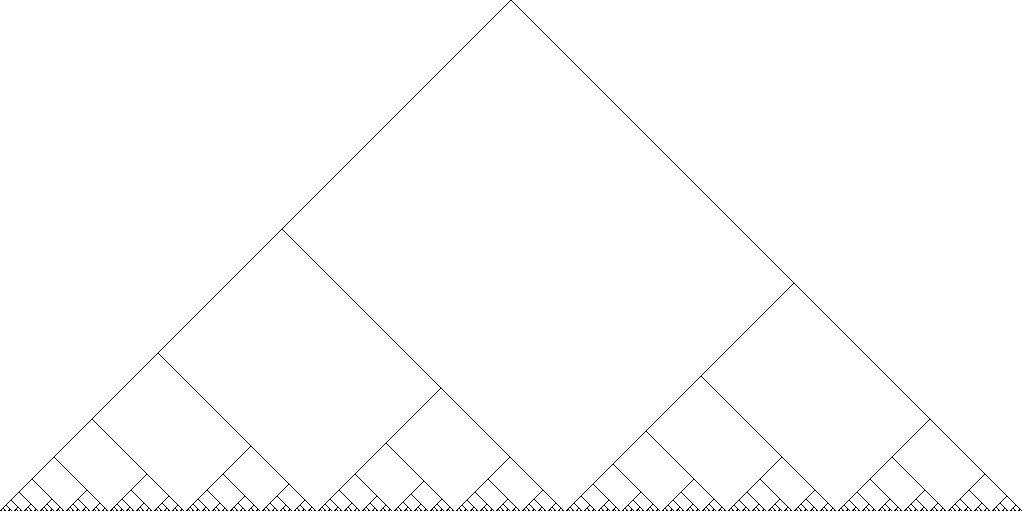
\includegraphics[width=0.8\textwidth]{optimal.png}
  \caption{Optimal strategy for $n=512,p=4.6,q=2.8$.}
  \label{fig:optimal}
\end{figure}

However, it is also possible to mathematically characterize the
optimal strategies. Since the optimal strategies for~$(p,q)$ are
symmetrical to those for~$(q,p)$, we may assume that~$p < q$. For
simplicity, we will also assume that $p$ and $q$ are integers: the
generalization to the case of rational $p$ and $q$ is
straightforward.

Let~$(u_m)$ be the sequence defined by~$u_{p+1} =
\dots = u_{p+q} = 1$ and~$u_m = u_{m-p} + u_{m-q}$, and~$f(n)$ be the
function defined by~$f(1) = 0$, $f(n) = f(u_{m}) + m(n - u_m)$
for all~$n \in [u_{m}, u_{m+1}]$. We check that $f$~satisfies the
recurrence relation
\begin{equation}\label{eq:recurrence-f}
f(u_m) = f(u_{m-p}) + f(u_{m-q}) + p u_{m-p} + q u_{m-q}.
\end{equation}

\begin{proposition}\label{prop:optimal-strategy}
A full strategy~$S$ is optimal if, and only if, it is canonical, both its left
and right branches~$S'$ and~$S''$ are optimal, and
\[ u_{m-q} \leq \abs{S'} \leq u_{m-q+1}, \quad
  u_{m-p} \leq \abs{S''} \leq u_{m-p+1}, \]
where $m$~is such that~$u_{m} \leq \abs{S} < u_{m+1}$. In this case, the
weight of~$S$ is~$f(\abs{S})$.
\end{proposition}

For example, in the case where~$p = 1$ and~$q = 2$, the sequence~$(u_m)$
is the sequence of Fibonacci numbers, starting at~$u_2 = 1$, $u_3 = 1$,
$u_4 = 2$..., and a strategy~$S$ with~$u_{m} \leq \abs{S} < u_{m+1}$ is
optimal if, and only if, the left and right branches~$S'$ and~$S''$
satisfy $u_{m-2} \leq \abs{S'} \leq u_{m-1}$ and~$u_{m-1} \leq \abs{S''} \leq
u_m$.

\begin{proof}
We prove this by induction on~$n = \abs{S}$. Let~$n = n' + n''$ with~$n',
n'' > 0$ and let~$S = S_{n',n''}$ be any canonical full strategy with optimal
left and right branches~$S'$, $S''$, such that~$\abs{S'} = n'$
and~$\abs{S''} = n''$. Then any optimal strategy is one of
the~$S_{n',n''}$. Therefore, we find them by looking at the sign
of~$\delta_n = (S_{n'+1,n''-1}) - (S_{n',n''})$.

Let~$m',m''$ be such that~$u_{m'} \leq n' < u_{m' + 1}$ and~$u_{m''} \leq
n'' < u_{m''+1}$. Using the induction hypothesis on~$S'$ and~$S''$, we
have $(S_{n',n''}) = f(n') + f(n'')  + n' q + n'' p$, and therefore
\begin{equation}
\delta_n \;=\; \begin{cases}
(m' + q) - (m'' + p),& \text{if $n'' \geq u_{m''} + 1$,}\\
(m' + q) - (m'' + p) + 1, &\text{if $n'' = u_{m''}$.}
\end{cases}
\end{equation}
We find that~$\delta_n \leq 0$ exactly when~$n' < u_{m-q+1}$ and~$n'' >
u_{m-p}$, and $\delta_n \geq 0$ exactly when~$n' \geq u_{m-q}$ and~$n''
\leq u_{m-p+1}$. The optimality condition follows from this.
It remains only to check that~$(S) = f(\abs{S})$: this results from
relation~(\ref{eq:recurrence-f}).
\end{proof}

In particular, there are in general several optimal strategies of a given
size. Moreover, with~$z$ being the (unique) root in~$[0,1]$ of the
equation~$z^p + z^q - 1 = 0$, this gives the asymptotic equivalents
\begin{eqnarray}
\abs{S'} &\sim& z^q \abs{S},\\
C_{p,q}(n) = (S) &\sim& -\frac{1}{\log z}\, n \log n.
\end{eqnarray}
The relative cost of an optimal stategy is therefore
asymptotically~$-\frac{2 \log 2}{\log (z^{p+q})}$ times the cost of
the balanced strategy. In the case where~$(p, q) = (4.6, 2.8)$, as in
Table~\ref{tab:counts} with~$\ell = 2$, this gives an improvement
of~2.1\% over the balanced strategy.

\subsection{Choice of the models}\label{subsec:montgomery}

At each phase of the key generation it is important to use models for
elliptic curves that offer the fastest formulas for doubling,
addition, isogeny computation and evaluation, etc.

To measure efficiency, we count the number of elementary operations in
$\FF_{p^2}$: we write $I,M,S$ for the costs of one inversion,
multiplication and squaring respectively, and we make the assumption
$S\le M\le I$. We neglect additions, subtractions and comparisons. We
refer to the Explicit Formulas Database (EFD)~\cite{efd} for operation
counts of elliptic point addition, doubling, etc. in various models
and coordinate systems. Contrary to the convention taken in the EFD,
we count multiplications by constants (other than small integers) as
ordinary multiplications.

Any curve used in our cryptosystem has group structure
$\left(\ZZ/(p\mp 1)\ZZ\right)^2$. Hence either the curve or its twist
has a point of order~$4$. Consequently, it is isomorphic to a twisted
Edwards curve and to a Montgomery curve~\cite{twisted-edwards}.

Twisted Edwards curves~\cite{twisted-edwards} have equation
\begin{equation}
  \label{eq:twisted-ed}
  E_{a,d}\;:\;ax^2+y^2=1+dx^2y^2.
\end{equation}
They have many interesting properties, but what interests us most is
their very efficient addition and doubling formulas.  Using projective
coordinates, one point addition costs $12M+1S$ and one point doubling
costs $4M+4S$. When one of the points is scaled to have $Z$-coordinate
equal to $1$, these costs drop to $11M+1S$ and $3M+4S$ respectively.

Montgomery curves~\cite{montgomery} have equation
\begin{equation}
  \label{eq:montgomery}
  M_{B,A}\;:\;By^2 = x^3 + Ax^2 + x.
\end{equation}
They have very efficient arithmetic on their Kummer line, i.e., by
representing points by the coordinates $(X:Z)$ where $x=X/Z$.  Using
this representation, a point can be doubled using $3M+2S$, or $2M+2S$
when it is scaled to have $Z$-coordinate equal to $1$.

The Kummer line identifies $P$ with $-P$; thus it is not possible to
add two distinct points. However it is still possible to perform what
is called \emph{differential addition}, i.e., adding points $P$ and
$Q$ for which the difference $P-Q$ is known. One differential addition
can be computed using $4M+2S$, or $3M+2S$ when the difference $P-Q$ is
scaled to have $Z$-coordinate equal to $1$.

By using doublings and differential additions, it is possible to
compute any scalar multiple of a point using a Montgomery
ladder~\cite{montgomery}. Also observe that since $P$ and $-P$
generate the same subgroup, isogenies can be defined and evaluated
correctly on the Kummer line. We shall give formulas for this
operation later.

It is shown in~\cite{twisted-edwards} that the twisted Edwards curve
$E_{a,d}$ is birationally equivalent to the Montgomery curve $M_{A,B}$
where
\begin{equation}
  A = \frac{2(a+d)}{a-d}, \qquad B = \frac{4}{a-d},
\end{equation}
and where the transformation is given by the following maps (in
affine coordinates)
\begin{equation}
  \label{eq:birational}
  \begin{aligned}
    \psi\;:\;E_{a,d}&\to M_{A,B},\\
    (x,y) &\mapsto \left(\frac{1+y}{1-y}, \frac{1+y}{(1-y)x}\right),
  \end{aligned}
  \qquad
  \begin{aligned}
    \psi^{-1}\;:\;M_{A,B}&\to E_{a,d},\\
    (x,y) &\mapsto \left(\frac{x}{y}, \frac{x-1}{x+1}\right).
  \end{aligned}
\end{equation}
Hence, after the models $E_{a,d}$ and $M_{A,B}$ are computed, points
in projective coordinates can be moved from one model to the other at
a cost of a few multiplications (and no inversions).

Now we detail the cost of each step of the key generation algorithm.

\subsubsection{Computing $\cyc{[m]P+[n]Q}$}\label{sssec:montgomery-ladder}

We have already mentioned two algorithms to compute the value of
$P+[m^{-1}n]Q$. One solution is to express the points $P$ and $Q$ in
projective Edwards coordinates and perform a double and add followed
by an addition. If we scale $Q$ to have $Z$-coordinate equal to $1$,
computing $[m^{-1}n]Q$ costs $9.5M+4.5S$ per bit on average.

Because addition by $P$ is performed last, this approach cannot
be used with points on the Montgomery curve in Kummer coordinates, but
we can use the ladder given in Algorithm~\ref{fig:ladder} instead. We
first compute $P-Q$ using point addition in full projective
coordinates (either by using the standard chord-and-tangent law, or by
using the equivalence with twisted Edwards curves). Then we scale $P$,
$Q$ and $P-Q$ to have $Z$-coordinate equal to $1$. We can now discard
the $Y$ coordinate and work on the Kummer line. At each iteration we
perform one doubling and two differential additions (with one of the
scaled points $P$, $Q$ and $P-Q$). The total cost of one iteration is
thus $9M+6S$.

In general the cost of one squaring is close to the cost of one
multiplication. Thus the ladder algorithm is slightly slower than
double-and-add. However the advantages of the ladder are SPA
resistance and an implementation simplified by not using Edwards
coordinates at all for key generation.

\subsubsection{Isogenies of Montgomery curves}\label{sssec:montgomery-isogeny}

The literature on efficient formulas for evaluating small degree
isogenies is much less extensive than for point multiplication. We now
give explicit formulas for isogenies of Montgomery curves, and
optimize the degree $2$ and $3$ cases. Our goal is to obtain the most
efficient formulas for isogeny evaluation, and thus we seek to avoid
inversions and square root computations as much as possible.

Let $E$ be the Montgomery curve defined by Eq.~\eqref{eq:montgomery}.
It has a point of order two $P_2=(0,0)$, and a point of order four
$P_4=(1,\sqrt{(A+2)/B})$---sometimes defined over a quadratic
extension---such that $[2]P_4=P_2$. Montgomery curves have twists of
the form $\tilde{y}=\sqrt{c}y$; these are isomorphisms when $c$ is a
square. The change of coordinates $\tilde{x}=x/B, \tilde{y}=y/B$
brings the curve $E$ to the Weierstrass form
\begin{equation}
  \label{eq:twisted}
  \tilde{y}^2 = \tilde{x}^3 + \frac{A}{B}\tilde{x}^2 + \frac{1}{B^2}\tilde{x},
\end{equation}
and the point $P_4$ to $P_4'=(1/B,\ldots)$. Conversely, given a
Weierstrass curve with equation
$\tilde{y}^2=\tilde{x}^3+a\tilde{x}^2+b\tilde{x}$, together with a
point $P_4=(1/\beta,\ldots)$---with its ordinate possibly lying in a
quadratic extension---such that $[2]P_4=(0,0)$, the change of
variables $\tilde{x}=x/\beta, \tilde{y}=y/\beta$ brings the curve to
the Montgomery form $\beta y^2=x^3+a\beta x^2 + x$.

Given a point $P\ne\pm P_4$ of order $4$, we will need to compute the
isomorphism of Montgomery curves that brings $[2]P$ in $(0,0)$ and $P$
in $(1,\ldots)$. Let $X$ be the abscissa of $P$ and $X_0$ the abscissa
of $[2]P$; by a straightforward calculation, we find that this
isomorphism is given by the map
\begin{equation}
  \label{eq:isomorphism}
  \begin{aligned}
    \iota : E &\to E',\\
    (x,y) &\mapsto \left(\frac{x-X_0}{X-X_0}, \frac{y}{X-X_0}\right),
  \end{aligned}
\end{equation}
and the new curve has equation
\begin{equation*}
  E' \;:\; \frac{B}{X-X_0}y^2 = x^3 + \frac{3X_0 + A}{X-X_0} x^2 + x.
\end{equation*}

By precomputing $1/(X-X_0)$, and sharing common subexpressions, the
above map can be evaluated on a point in full projective
coordinates using $3M$ operations, or $2M$ using Kummer
coordinates.

Let $G$ be a subgroup of the Montgomery curve $E$ of odd cardinality
$\ell$ and let $h$ be the degree $(\ell-1)/2$ polynomial vanishing on
the abscissas of $G$. With a twist $y=\tilde{y}/\sqrt{B}$, we can put
$E$ in the form
\begin{equation*}
  E \;:\; \tilde{y}^2 = \tilde{x}^3 + A\tilde{x}^2 +\tilde{x},
\end{equation*}
and this does not change the abscissas of $G$ nor the polynomial
$h$. Now, composing the twist with V\'elu's formulas gives an isogeny
\begin{equation*}
  \begin{aligned}
    \phi : E &\to E/G,\\
    (x,y) &\mapsto \left(\frac{g(x)}{h(x)^2}, y\sqrt{B}\left(\frac{g(x)}{h(x)^2}\right)'\right).
  \end{aligned}
\end{equation*}

We now need to express $E/G$ in Montgomery form. Because $\ell$ is
odd, the point $(0,0)$ of $E$ is sent to a point of order two in
$E/G$, and the change of variables
$\tilde{x}=x-g(0)/h(0)^2$ brings this point to $(0,0)$.

Now, $\phi(P_4)$ is a point of order four lying above $(0,0)$ (possibly
in a quadratic extension). Its abscissa is rational and is given by
\begin{equation}
  \frac{1}{\beta} = \frac{g(1)}{h(1)^2} - \frac{g(0)}{h(0)^2},  
\end{equation}
so we further apply the change of variables
$\tilde{x}=\bar{x}/\beta,\tilde{y}=\bar{x}/\beta$ to obtain a
Montgomery curve. Finally, we have to twist back the model in order to
obtain a curve isogenous over the base field: the twist $\bar{y} =
y\sqrt{B}$ cancels with the first one and leaves us with
square-root-free formulas.

Given $h$ as input, the cost of evaluating the whole path is $O(\ell)$
operations in the base field, using the formula in
\cite[Proposition~4.1]{Bostan} to evaluate $g/h$.

Let now $P$ be a $3$-torsion point, let $G=\{0,P,-P\}$ and let $X$ be
the abscissa of $P$ (and $-P$). If we specialize the formula to the
case $\ell=3$, we have $h = x - X$ and
\begin{equation}
  \label{eq:3-isogeny}
  \begin{aligned}
    \phi : E &\to E/G,\\
    (x,y) &\mapsto \textstyle{\left(
      \frac{x\left(x - \frac{1}{X}\right)^2}{(x-X)^2}X^2,\;
      y\frac{\left(x-\frac{1}{X}\right)\left(\left(x-\frac{1}{X}\right)(x-X)+2x\left(\frac{1}{X}-X\right)\right)}{(x-X)^3}X^2
    \right),}
  \end{aligned}
\end{equation}
and the curve $E/G$ has equation
\begin{equation*}
  E/G \;:\; BX^2y^2 = x^3 + \left(A+\frac{6}{X}-6X\right)X^2x^2 + x.
\end{equation*}

By precomputing $X$ and $X^2$, and sharing common subexpressions, the
above isogeny can be evaluated on a point in full projective
coordinates using $11M+2S$ operations, or $4M + 2S$ using Kummer
coordinates.

When $\ell$ is even, things get more complicated. Recall that
$P_2=(0,0)$ and $P_4=(1,\sqrt{(A+2)/B})$. The isogeny of degree $2$
vanishing on $P_2$ and mapping $P_4$ to $(0,0)$ is readily seen as
being
\begin{align}
  \label{eq:isogeny-2}
  &F \;:\;  By^2 = x^3 + (A+6)x^2 + 4(2+A)x,\\
  &\begin{aligned}
    \phi : E &\to F,\\
    (x,y) &\mapsto \left(\frac{(x-1)^2}{x}, y\left(1 - \frac{1}{x^2}\right)\right).
  \end{aligned}
\end{align}
It is not immediately evident how to put $F$ in Montgomery form
without computing square roots. Let $P_8$ be a point satisfying
$[2]P_8=P_4$. Then we have $\phi(P_8)=(2\sqrt{2+A},\ldots)$, and $F$ can be
put in the form
\[\frac{B}{2\sqrt{2+A}}y^2 = x^3 + \frac{A+6}{2\sqrt{2+A}}x^2 + x,\]
with the point $(1,\ldots)$ being the image of $P_8$.  Any other
isogeny of degree $2$ can be treated by applying
Eq.~\eqref{eq:isomorphism} to move the generator of the kernel in
$(0,0)$.

By precomputing $1/\phi(P_8)$, and sharing common subexpressions, the
above isogeny can be evaluated on a point in full projective
coordinates using $5M+3S$ operations, or $2M+S$ using Kummer
coordinates. Unfortunately, this formula takes no square roots only if
an $8$-torsion point above $P_2$ is known.


Alternatively, $\phi$ and $F$ being as before, we consider the isogeny
$\psi:F\to F/\cyc{(0,0)}$ given by
\begin{align}
  \label{eq:isogeny-4}
  &G \;:\;  \frac{B}{2-A}y^2 = x^3 - 2\frac{A+6}{2-A}x^2 + x,\\
  &\begin{aligned}
    \psi : F &\to G,\\
    (x,y) &\mapsto \left(\frac{1}{2-A}\frac{(x+4)(x+(A+2))}{x}, \frac{y}{2-A}\left(1 - \frac{4(2+A)}{x^2}\right)\right).
  \end{aligned}
\end{align}
Then $\phi_4 = \psi\circ\phi$ is an isogeny of degree four
$\phi_4\colon E\to
E/\cyc{P_4}$, and the point $\left(1,\sqrt{-4(A+2)/B}\right)$ of $G$
generates the kernel of the dual isogeny $\hat{\phi}_4$. Any other
isogeny of degree $4$ can be treated by applying
Eq.~\eqref{eq:isomorphism} to move the kernel point to $(1,\ldots)$.

By precomputing $1/(2-A)$, and sharing common subexpressions, the
isogeny $\phi_4$ can be evaluated on a point in full projective
coordinates using $10M+4S$ operations, or $4M+S$ using Kummer
coordinates.

Unfortunately, this formula cannot be applied twice to obtain a degree
$16$ cyclic isogeny: indeed, a double application yields the
multiplication-by-$4$ isogeny. If a chain of degree $4$ isogenies is
wanted, as for the algorithm in Subsection~\ref{sssec:isogeny}, this
formula must be combined with the isomorphism in
Eq.~\eqref{eq:isomorphism}.

Isogenies of composite smooth degree are computed by composing small
degree isogenies as discussed in Subsection~\ref{sssec:isogeny}. We
focus on the fine tuning of this algorithm when the small isogenies
have degrees $2,3$ and $4$.

It is important to remark that, after a generator $R$ of the kernel of
the isogeny has been computed, the algorithm does not use its ordinate
at all: indeed, all the previous formulas for small degree isogenies
only use the abscissas of the kernel points. Hence, we can throw away
the ordinate of $R$ altogether and only use scalar multiplication and
isogeny evaluation formulas for points in Kummer
coordinates.

As usual, some more care must be taken when computing cyclic isogenies
of degree $2^e$. In principle, one could compose either degree $2$
(Eq.~\ref{eq:isogeny-2}) or degree $4$ (Eq.~\ref{eq:isogeny-4})
isogenies; however we have already pointed out some caveats:

\begin{itemize}
\item Both equations require the kernel point to be moved to some
  specific coordinates. This can be achieved using the isomorphism in
  Eq.~\eqref{eq:isomorphism}.
\item After the first change of variables, Eq.~\eqref{eq:isogeny-2}
  can be repeatedly chained with itself; however, from a point of
  order $2^e$ only $e-2$ degree $2$ isogenies can be computed this
  way, because the formula requires the knowledge of a point of order $8$.
\item Eq.~\eqref{eq:isogeny-4} cannot be directly chained with itself
  to compute a cyclic isogeny of degree $4^e$. It must be composed,
  instead, with Eq.~\eqref{eq:isomorphism} at each step.
\end{itemize}

Having this in mind, two obvious strategies to compute degree $2^e$
isogenies are:

\begin{enumerate}
\item Use degree $2$ isogenies as much as possible; use one degree $4$
  isogenies for the last two steps.
\item Use one degree $2$ isogeny if $e$ is odd, then use only degree
  $4$ isogenies composed with isomorphisms.
\end{enumerate}

Table~\ref{tab:strategies} below suggests that the second stragegy
yields a very small improvement over the first. The experiments of
Section~\ref{sec:imp} show that operations not accounted for in this
analysis might give a greater advantage to the second
strategy. However, for lack of time, we only implemented the first
one.

Finally, it should be noted that both approaches, if implemented as
described above, leak two bits of security. Indeed, the point
$(1,\ldots)$ of the image curve is a point of order $4$ in the kernel
of the dual of the computed isogeny (the secret). It is easy to mask
this by taking a random change of coordinates, thus in the security
analysis of Section~\ref{sec:security} we will assume that such
countermeasure has been applied. However, for practical purposes, we
found this more costly than simply adding two bits of security and
letting the information leak.

Table~\ref{tab:counts} summarizes the costs of the isogeny evaluation
and scalar multiplication formulas in light of these remarks. Because
squaring in $\FF_{p^2}$ is faster than multiplication, we also report
the cost obtained by taking $S=0.8M$ (a factor that roughly
approximates the fact that squaring requires $2$ multiplications in
$\FF_p$ instead of $3$).

Table~\ref{tab:strategies} compares the total cost of isogeny
evaluations and scalar multiplications in a balanced and an optimal
strategy for $\ell=2,3,4$, based on the costs given in
Table~\ref{tab:counts}, at the classical 256-bit security level (see
Section~\ref{sec:security} for our complexity assumptions). We make the following observations, backed up by the benchmarks in Section~\ref{sec:imp}:
\begin{itemize}
\item There may be a small advantage (less than $2\%$) in using
  isogenies of degree $4$ instead of $2$;
\item The gain in using an optimal strategy instead of a balanced one
  is consistent with the predictions of
  Subsection~\ref{sssec:isogeny};
\item The difference between $2^e$ and $3^e$ isogenies is more
  significant (about $20\%$), suggesting that degree $2^e$ isogenies
  may be preferable for constrained devices.
\end{itemize}

\begin{table}[t]
  \centering
  \caption{Comparative costs for multiplication and isogeny evaluation in projective Kummer coordinates, in number of multiplications and squarings, and assuming $S=0.8M$.}
  \label{tab:counts}
  \begin{tabular}{ l @{\hspace{1ex}} | *{3}{@{\hspace{1em}} r} }
    $\ell$ & $2$ & $3$ & $4$ \\
    \hline
    Isogeny & $2M+S$ & $4M+2S$ & $6M+S$\\
            &  $2.8$ &   $5.6$ &  $6.8$\\
    \hline
    Multiplication & $3M+2S$ & $7M+4S$ & $6M+4S$\\
                   &   $4.6$ &  $10.2$ &   $9.2$
  \end{tabular}
\end{table}


\begin{table}[t]
  \centering
  \caption{Comparative costs of the balanced and the optimal strategies for computing a degree $2^{514}$ ($\ell=2,4$) or $3^{323}$ ($\ell=3$) isogeny, assuming $S=0.8M$.}
  \label{tab:strategies}
  \begin{tabular}{ l | *{3}{r} | *{3}{r} }
    & \multicolumn{3}{c|}{optimal strategy} & \multicolumn{3}{c}{balanced strategy}\\
    $\ell$ & $2$ & $3$ & $4$ & $2$ & $3$ & $4$\\
    \hline
    Isogenies       & $2741$    & $1610$    & $1166$    & $2323$    & $1430$    & $1033$ \\
    Multiplications & $1995$    & $1151$    & $921$     & $2307$    & $1288$    & $1025$ \\
    Total cost      & $16852$ & $20756$ & $16402$ & $17117$ & $21146$ & $16454$
  \end{tabular}
\end{table}


\section{Complexity assumptions}\label{sec:security}

As before, let $p$ be a prime of the form $\ell_A^{e_A}
\ell_B^{e_B}\cdot f \pm 1$, and fix a supersingular curve $E_0$ over
$\FF_{p^2}$ together with bases $\{P_{A},Q_{A}\}$ and
$\{P_{B},Q_{B}\}$ of $E_0[\ell_A^{e_A}]$ and $E_0[\ell_B^{e_B}]$
respectively. In analogy with the case of isogenies over ordinary
elliptic curves, we define the following computational problems,
adapted for the supersingular case:

\begin{problem}[Decisional Supersingular Isogeny (DSSI) problem] Let
  $E_A$ be another supersingular curve defined over
  $\FF_{p^2}$. Decide whether $E_A$ is $\ell_A^{e_A}$-isogenous to
  $E_0$.
\end{problem}

\begin{problem}[Computational Supersingular Isogeny (CSSI) problem]
Let the map $\phi_A \colon E_0 \to E_A$ be an isogeny whose kernel is
$\cyc{[m_A]P_A+[n_A]Q_A}$, where $m_A$ and $n_A$ are chosen at random
from $\ZZ/\ell_A^{e_A}\ZZ$ and not both divisible by $\ell_A$.  Given
$E_A$ and the values $\phi_A(P_B)$, $\phi_A(Q_B)$, find a generator
$R_A$ of $\cyc{[m_A]P_A+[n_A]Q_A}$.
\end{problem}

We remark that given a generator $R_A = [m_A]P_A+[n_A]Q_A$, it is easy
to solve for $(m_A,n_A)$, since $E_0$ has smooth order and thus
extended discrete logarithms are easy in $E_0$~\cite{teske-ph}.

\begin{problem}[Supersingular Computational Diffie-Hellman
    (SSCDH) problem] Let $\phi_A \colon E_0 \to E_A$ be an isogeny
  whose kernel is equal to $\cyc{[m_A]P_A+[n_A]Q_A}$, and let $\phi_B \colon
  E_0 \to E_B$ be an isogeny whose kernel is
  $\cyc{[m_B]P_B+[n_B]Q_B}$, where $m_A,n_A$ (respectively $m_B,n_B$)
  are chosen at random from $\ZZ/\ell_A^{e_A}\ZZ$ (respectively
  $\ZZ/\ell_B^{e_B}\ZZ$) and not both divisible by $\ell_A$ (respectively
  $\ell_B$). Given the curves $E_A,$ $E_B$ and the points
  $\phi_A(P_B),$ $\phi_A(Q_B),$ $\phi_B(P_A),$ $\phi_B(Q_A)$, find the
  $j$-invariant of $E_0/\cyc{[m_A]P_A+[n_A]Q_A ,[m_B]P_B+[n_B]Q_B}$.
\end{problem}

\begin{problem}[Supersingular Decision Diffie-Hellman (SSDDH)
    problem] Given a tuple sampled with probability $1/2$ from one of
  the following two distributions:
\begin{itemize} 
\item $(E_A, \phi_A(P_B), \phi_A(Q_B), E_B, \phi_B(P_A), \phi_B(Q_A),
  E_{AB})$, wherein the quantities $E_A,$ $\phi_A(P_B),$ $\phi_A(Q_B),$ $E_B,$
  $\phi_B(P_A),$ and $\phi_B(Q_A)$ are as in the SSCDH problem and \[E_{AB} \iso
  E_0/\cyc{[m_A]P_A+[n_A]Q_A ,[m_B]P_B+[n_B]Q_B},\]
\item $(E_A, \phi_A(P_B), \phi_A(Q_B), E_B, \phi_B(P_A), \phi_B(Q_A),
  E_C)$, wherein the quantities $E_A,$ $\phi_A(P_B),$ $\phi_A(Q_B),$ $E_B,$
  $\phi_B(P_A),$ and $\phi_B(Q_A)$ are as in the SSCDH problem and \[E_{C} \iso
  E_0/\cyc{[m_A']P_A+[n_A']Q_A ,[m_B']P_B+[n_B']Q_B},\] where
  $m_A',n_A'$ (respectively $m_B',n_B'$) are chosen at random from
  $\ZZ/\ell_A^{e_A}\ZZ$ (respectively $\ZZ/\ell_B^{e_B}\ZZ$) and not both
  divisible by $\ell_A$ (respectively $\ell_B$),
\end{itemize}
determine from which distribution the tuple is sampled.
\end{problem}

The ordinary case analogue of the following problem is trivially
solvable in polynomial time. Its supposed difficulty in the
supersingular case is at the heart of the security of our
identification scheme.

\begin{problem}[Decisional Supersingular Product (DSSP) problem]
  Given a degree $\ell_A^{e_A}$ isogeny $\phi:E_0\to E_3$ and a
  tuple sampled with probability $1/2$ from one of the following two
  distributions:
  \begin{itemize} 
  \item $(E_1,E_2,\phi')$, where the product $E_1\times E_2$ is chosen
    at random among those $\ell_B^{e_B}$-isogenous to $E_0\times E_3$,
    and where $\phi':E_1\to E_2$ is an isogeny of degree
    $\ell_A^{e_A}$, and
  \item $(E_1,E_2,\phi')$, where $E_1$ is chosen at random among the
    curves having the same cardinality as $E_0$, and $\phi':E_1\to
    E_2$ is a random isogeny of degree $\ell_A^{e_A}$,
  \end{itemize}
  determine from which distribution the tuple is sampled.
\end{problem}

We conjecture that these problems are computationally infeasible, in
the sense that for any polynomial-time solver algorithm, the advantage
of the algorithm is a negligible function of the security parameter
$\log p$. The resulting security assumptions are referred to as the
DSSI assumption, CSSI assumption, etc.


\subsection{Hardness of the underlying
  assumptions}\label{subsec:hardness}

Given a CSSI (respectively, SSCDH) solver, it is trivial to solve
SSCDH (respectively, SSDDH). It is also trivial to solve SSDDH given a
DSSI solver. There are no known reductions in the other direction, and
given that the corresponding question of equivalence for discrete
logarithms and Diffie-Hellman has not yet been completely resolved in
all cases, it is reasonable to assume that the question of equivalence
of CSSI, SSCDH, and SSDDH is at least hard to resolve. For the
purposes of this discussion, we will presume that DSSI and CSSI are
equivalent to SSDDH. Concerning DSSP, there is an evident reduction to
DSSI. However, it seems reasonable to assume that DSSP is easier than the
latter.

In the context of cryptography, the problem of computing an isogeny
between isogenous supersingular curves was first considered by
Galbraith~\cite{Gal} in 1999. The first published cryptographic
primitive based on supersingular isogeny graphs is the hash function
proposal of Charles et al.~\cite{CGL}, which remains unbroken to date
(the cryptanalysis of~\cite{quis} applies only to the LPS graph-based
hash function from~\cite{CGL}, and not to the supersingular isogeny
graph-based hash functions). The fastest known algorithm for finding
isogenies between supersingular curves in general takes $O(\sqrt{p}
\log^2 p)$ time~\cite[\S 5.3.1]{CGL}; however our problem is less
general because the degree of the isogeny is known in advance and is
smooth. In addition, the distribution of isogenous
  curves obtained
from taking kernels of the form $\cyc{[m_A]P_A+[n_A]Q_A}$ is not quite
uniform: a simple calculation against Proposition~\ref{prop:mixing}
indicates that a sequence of $e_A$ isogenies of degree $\ell_A$ falls
short of the length needed to ensure uniform mixing, regardless of the
value of $p$. Since we are the first to propose using isogenies of
this type, there is no existing literature addressing the security
of the isogenies of the special form that we propose.

There are easy exponential attacks against DSSI and CSSI that improve
upon exhaustive search. To find an isogeny of degree $\ell_A^{e_A}$
between $E$ and $E_A$, an attacker builds two trees of all curves
isogenous to $E$ (respectively, $E_A$) via isogenies of degree
$\ell_A^{e_A/2}$. Once the trees are built, the attacker tries to find
a curve lying in both trees. Since the degree of the isogeny $\phi_A$
is $\sim\sqrt{p}$ (much shorter than the size of the isogeny graph),
it is unlikely that there will be more than one isogeny path---and
thus more than one match---from $E$ to $E_A$. Given two functions
$f:A\to C$ and $g:B\to C$ with domain of equal size, finding a pair
$(a,b)$ such that $f(a)=g(b)$ is known as the \emph{claw problem} in
complexity theory. The claw problem can obviously be solved in $O(|A|
+ |B|)$ time and $O(|A|)$ space on a classical computer by building a
hash table holding $f(a)$ for any $a\in A$ and looking for hits for
$g(b)$ where $b\in B$. This gives a $O(\ell_A^{e_A/2})=O(\sqrt[4]{p})$
classical attack against our cryptosystems. With a quantum computer,
one can do better using the algorithm in~\cite{tani}, which has
complexity $O(\sqrt[3]{|A||B|})$, thus giving an
$O(\ell_A^{e_A/3})=O(\sqrt[6]{p})$ quantum attack against our
cryptosystems. These complexities are optimal for a black-box claw
attack~\cite{zhang}.

We consider the question of whether the auxiliary data points
$\phi_A(P_B)$ and $\phi_A(Q_B)$ might assist an adversary in
determining $\phi_A$. Since $(P_B,Q_B)$ forms a basis for
$E_0[\ell_B^{e_B}]$, the values $\phi_A(P_B)$ and $\phi_A(Q_B)$ allow
the adversary to compute $\phi_A$ on all of $E_0[\ell_B^{e_B}]$. This
is because any element of $E_0[\ell_B^{e_B}]$ is a (known) linear
combination of $P_B$ and $Q_B$ (known since extended discrete
logarithms are easy~\cite{teske-ph}). However, there does not appear
to be any way to use this capability to determine $\phi_A$. Even on a
quantum computer, where finding abelian hidden subgroups is easy,
there is no hidden subgroup to find, since $\phi_A$ has degree
$\ell_A^{e_A}$, and thus does not annihilate any point in
$E_0[\ell_B^{e_B}]$ other than the identity. Of course, if one could
evaluate $\phi_A$ on arbitrary points of $E_0[\ell_A^{e_A}]$, then a
quantum computer could easily break the scheme, and indeed in this case the
scheme is also easily broken classically by using a few calls to the
oracle to compute a generator of the kernel of the dual isogeny 
$\hat{\phi}_A$. However, it does not seem possible to translate the values of
$\phi_A$ on $E_0[\ell_B^{e_B}]$ into values on $E_0[\ell_A^{e_A}]$.

For both ordinary and supersingular curves, there is a natural
bijection between isogenies (up to isomorphism) and (left) ideals in
the endomorphism ring. In the ordinary case the endomorphism ring is
commutative, and ideal classes form a finite abelian group. This
property has been used by Childs et al.~\cite{CJS} to solve the
ordinary analogue of CSSI in quantum subexponential time. It is
natural to ask whether their algorithm can be adapted to the
supersingular setting. Here the
endomorphism ring is a maximal order in a noncommutative quaternion
algebra, and the left ideal classes do not form a group at all (though
they do
form a groupoid). Since the algorithm of Childs et al. depends
crucially on the properties of abelian groups, we believe that no
reasonable variant of this strategy would apply.

The same correspondence between isogenies and ideals can be applied to
DSSP. Indeed, deciding DSSP amounts to deciding whether the ideals
$S,S'$ associated to $\phi,\phi'$ are conjugated, i.e., whether there
exists a left ideal $R\in\End(E_0)$ such that $S=RS'R^{-1}$. Although
it can be hoped that deciding conjugacy of ideal classes in the
quaternion algebra $\QQ_{p,\infty}$ is feasible, we are still faced
with the problem that the best known algorithms to compute the
endomorphism rings of supersingular curves are exponential in $\log
p$~\cite{Kohel,cervino04,belding08-thesis}. Hence, we deem DSSP secure
given the current knowledge.

The fact that it is possible to obtain a zero-knowledge identification
scheme from CSSI comes as no surprise, since it is well known that a
zero-knowledge protocol can be obtained from any problem in
NP~\cite{goldreich+micali+widgerson91}. Nevertheless, the generic
construction is not very efficient, and many efforts have been made to
obtain efficient \emph{ad-hoc} schemes from NP-complete
problems~\cite{shamir89-pkp,stern94-CLE,stern94-SD,pointcheval95-pp}. While
the security of most of these schemes is based on two solid
assumptions, namely that P $\ne$ NP and that \emph{secure commitment
  schemes} exist, our identification scheme stands on a much
weaker ground: the CSSI and DSSP problems. As performances go, it is
reasonable to assume that our scheme will be some orders of magnitude
slower than the best zero-knowledge protocols. We can thus conclude
that our scheme is of a purely theoretical and pedagogical interest.
Yet it is remarkable that an efficient identification scheme based on
graphs of supersingular isogenies simply exists, while the analogous
construction for ordinary curves is trivially broken and no other
identification scheme is currently known to work in that
case~\cite{Stol}.

\section{Security proofs}\label{sec:proof}



In this section we state formal security reductions relating the
security of our protocols to the hardness of the appropriate
underlying isogeny computation problem. The security proofs are
routine, but tedious, and contain little original contribution on
our part. For this reason, we only prove a representative selection
of our theorems.

The statements of the theorems are as follows:

\begin{theorem}\label{thm:kep-proof}
If the SSDDH assumption holds, then the key-agreement protocol of
Section~\ref{subsec:kep} is session-key secure in the
authenticated-links adversarial model of Canetti and
Krawczyk~\cite{canetti}.
\end{theorem}
\begin{theorem}\label{thm:pk-proof}
If the SSDDH assumption holds, and the hash function family
$\mathcal{H}$ is entropy-smoothing, then the public-key cryptosystem
of Section~\ref{subsec:pk} is IND-CPA.
\end{theorem}
\begin{theorem}\label{thm:zk-proof}
  Under the CSSI and DSSP assumptions, the identification scheme of
  Section~\ref{subsec:zk} is zero-knowledge.
\end{theorem}

\subsection{Proof of Theorem~\ref{thm:kep-proof}}\label{subsec:zkp-proof}

The proofs of Theorems~\ref{thm:kep-proof} and~\ref{thm:pk-proof} are
easily adapted from the corresponding proofs given by
Stolbunov~\cite{stolbunov-red}. As an illustration of the proof
techniques, we provide a proof of Theorem~\ref{thm:kep-proof}.

We recall the definition of session-key security in the
authenticated-links adversarial model of Canetti and
Krawczyk~\cite{canetti}. We consider a finite set of \emph{parties}
$P_1, P_2, \ldots, P_n$ modeled by probabilistic Turing machines.  The
adversary $\mathcal{I}$, also modeled by a probabilistic Turing
machine, controls all communication, with the exception that the
adversary cannot inject or modify messages (except for messages from
corrupted parties or sessions), and any message may be delivered at
most once. Parties give outgoing messages to the adversary, who has
control over their delivery via the \textsf{Send} query. Parties are
activated by \textsf{Send} queries, so the adversary has control over
the creation of protocol sessions, which take place within each party.
Two sessions $s$ and $s'$ are \emph{matching} if the outgoing messages
of one are the incoming messages of the other, and vice versa.

We allow the adversary black-box access to the queries
$\mathsf{SessionStateReveal}$, $\mathsf{SessionKeyReveal}$, and
$\mathsf{Corrupt}$. The $\mathsf{SessionStateReveal}(\mathfrak{s})$
query allows the adversary to obtain the contents of the session
state, including any secret information. The query is noted and
$\mathfrak{s}$ produces no further output.  The
$\mathsf{SessionKeyReveal(\mathfrak{s})}$ query enables the adversary
to obtain the session key for the specified session $\mathfrak{s}$, so
long as $\mathfrak{s}$ holds a session key. The
$\mathsf{Corrupt(P_i)}$ query allows the adversary to take over the
party $P_i$, i.e.,\ the adversary has access to all information in
$P_i$'s memory, including long-lived keys and any session-specific
information still stored. A corrupted party produces no further
output. We say a session $\mathfrak{s}$ with owner $P_i$ is
\emph{locally exposed} if the adversary has issued
$\mathsf{SessionKeyReveal(\mathfrak{s})}$,
$\mathsf{SessionStateReveal(\mathfrak{s})}$, or
$\mathsf{Corrupt(P_i)}$ before $\mathfrak{s}$ is expired. We say
$\mathfrak{s}$ is \emph{exposed} if $\mathfrak{s}$ or its matching
session have been locally exposed, and otherwise we say $\mathfrak{s}$
is \emph{fresh}.

We allow the adversary $\mathcal{I}$ a single
$\mathsf{Test(\mathfrak{s})}$ query, which can be issued at any stage
to a completed, fresh, unexpired session $\mathfrak{s}$. A bit $b$ is
then picked at random. If $b=0$, the test oracle reveals the session
key, and if $b=1$, it generates a random value in the key
space. $\mathcal{I}$ can then continue to issue queries as desired,
with the exception that it cannot expose the test session. At any
point, the adversary can try to guess $b$. Let
$\operatorname{GoodGuess}^{\mathcal{I}}(k)$ be the event that
$\mathcal{I}$ correctly guesses $b$, and define \[
\operatorname{Advantage}^{\mathcal{I}}(k) = \max \left\{0, \left \vert
\operatorname{Pr}[\operatorname{GoodGuess}^{\mathcal{I}}(k)] - \frac 1
2 \right \vert \right\},\] where $k$ is a security parameter.

The definition of security is as follows:

\begin{definition}\label{def:kep}
A key exchange protocol $\Pi$ in security parameter $k$ is said to be
\emph{session-key secure} in the authenticated-links adversarial model
of Canetti and Krawczyk if for any polynomial-time adversary $\mathcal{I}$,
\begin{enumerate}
\item If two uncorrupted parties have completed matching sessions,
  these sessions produce the same key as output;
\item $\operatorname{Advantage}^{\mathcal{I}}(k)$ is negligible.
\end{enumerate}
\end{definition}

\begin{algorithm}[t]
\caption{SSDDH distinguisher}
\label{alg:distinguisher}
\begin{algorithmic}[1]
\REQUIRE $E_A, E_B, \phi_A(P_B), \phi_A(Q_B), \phi_B(P_A),
\phi_B(Q_A), E$
\STATE $r \stackrel{R}{\leftarrow} \{1,\ldots,k\}$, where $k$ is an
upper bound on the number of sessions activated by $\mathcal{I}$ in any
interaction.
\STATE Invoke $\mathcal{I}$ and simulate the protocol to $\mathcal{I}$, except for the
$r$-th activated protocol session.
\STATE For the $r$-th session, let Alice send $A$, $i$, $E_A$, $\phi_A(P_B)$,
$\phi_A(Q_B)$ to Bob, and let Bob send $B$, $i$, $E_B$, $\phi_B(P_A)$,
$\phi_B(Q_A)$ to Alice, where $i$ is the session identifier.
\IF{the $r$-th session is chosen by $\mathcal{I}$ as the test session}
\STATE Provide $\mathcal{I}$ as the answer to the test query.
\STATE $d \leftarrow \mathcal{I}$'s output.
\ELSE
\STATE $d \stackrel{R}{\leftarrow}\{0,1\}$.
\ENDIF
\ENSURE $d$

\end{algorithmic}
\end{algorithm}

\begin{proof}[Proof of Theorem~\ref{thm:kep-proof}]
We adapt the proof given by Canetti and Krawczyk~\cite[\S
  5.1]{canetti} for two-party Diffie-Hellman over $\ZZ_q^*$. A similar
strategy was used by Stolbunov~\cite{stolbunov-red} in the case of
ordinary elliptic curves.

It has been shown in Section~\ref{sec:kep} that two uncorrupted
parties in matching sessions output the same session key, and thus the
first part of Definition~\ref{def:kep} is satisfied. To show that the
second part of the definition is satisfied, assume that there is a
polynomial-time adversary $\mathcal{I}$ with a non-negligible advantage
$\varepsilon$. We claim that Algorithm~\ref{alg:distinguisher} forms a
polynomial-time distinguisher for SSDDH having non-negligible
advantage.

To prove the claim, we must show that
Algorithm~\ref{alg:distinguisher} has non-negligible advantage (it is
clear that it runs in polynomial time). We consider separately the
cases where the $r$-th session is (respectively, is not) chosen by
$\mathcal{I}$ as the test session. If the $r$-th session is not the
test session, then Algorithm~\ref{alg:distinguisher} outputs a random
bit, and thus its advantage in solving the SSDDH is $0$. If the
$r$-th session is the test session, then $\mathcal{I}$ will succeed
with advantage $\varepsilon$, since the simulated protocol provided to
$\mathcal{I}$ is indistinguishable from the real protocol. Since the
latter case occurs with probability $1/k$, the overall advantage of
the SSDDH distinguisher is $\varepsilon/k$, which is non-negligible.
\end{proof}



\subsection{Proof of Theorem~\ref{thm:zk-proof}}

Using classical techniques from
\cite{goldreich+micali+widgerson91,feige+fiat+shamir88}, the theorem
is proved in three steps, known by the names of \emph{completeness},
\emph{soundness} and \emph{zero-knowledge}.

\begin{proof}[Proof of Theorem~\ref{thm:zk-proof} (sketch)]
  Completeness is obvious: using the algorithms of
  Section~\ref{sec:alg}, Peggy can always compute the
  diagram~\eqref{eq:zk} in polynomial time and make Vic accept.

  To prove soundness, we let Charles be any polynomially bounded
  adversary capable of convincing Vic with a non-negligible
  probability. We use Charles as a black-box of which we can control
  the random coin tosses. By restarting it a polynomial number of
  times with the same random input, and by asking each time a different
  set of questions, we learn with overwhelming probability a diagram
  \begin{equation}
    \label{eq:zk1-soundness}
    \begin{tikzpicture}[xscale=2,yscale=1.5,baseline=(current bounding box.east)]
      \node(0) at (0,0) {$E$};
      \node(S) at (1,0) {$E/\cyc{S}$};
      \node(R) at (0,-1) {$E/\cyc{R}$};
      \node(SR) at (1,-1) {$E/\cyc{S,R}$};
            \path[->] (0) edge node[auto,swap] {$\psi$} (R);
      \path[->] (S) edge node[auto] {$\psi'$} (SR);
      \path[->] (R) edge node[auto] {$\phi'$} (SR);
    \end{tikzpicture}
  \end{equation}

  It is then straightforward to compute the secret. Let $R$ be a
  generator of the kernel of $\phi'$. Using the theorem of the dual
  isogeny it is easy to compute $\hat{\psi}$, then
  $\cyc{\hat{\psi}(R)}$ is the kernel of an isogeny $E\to E/\cyc{S}$
  of degree $\ell_A^{e_a}$. This contradicts the CSSI assumption.

  To prove zero-knowledge, we use a \emph{cheating verifier} (CV) as a
  black-box to construct a \emph{simulator} (S). At each iteration, S
  makes a (uniformly) random guess at what the next question by V will
  be.

  If S guesses $b=0$, it chooses a random primitive
  $\ell_B^{e_B}$-torsion point $R\in E$ and computes $\phi(R)$ (recall
  that the action of $\phi$ on $E[\ell_B^{e_B}]$ is part of the public
  data). Then it constructs the isogenies $\psi:E\to E/\cyc{R}$ and
  $\psi':E/\cyc{S}\to E/\cyc{S,R}$
  \begin{equation}
    \label{eq:zk2-vertical}
    \begin{tikzpicture}[xscale=2,yscale=1.5,baseline=(current bounding box.east)]
      \node(0) at (0,0) {$E$};
      \node(S) at (1,0) {$E/\cyc{S}$};
      \node(R) at (0,-1) {$E/\cyc{R}$};
      \node(SR) at (1,-1) {$E/\cyc{S,R}$};
      \path[->,dashed] (0) edge node[auto] {$\phi$} (S);
      \path[->] (0) edge node[auto,swap] {$\psi$} (R);
      \path[->] (S) edge node[auto] {$\psi'$} (SR);
    \end{tikzpicture}
  \end{equation}
  and sends $E_1=E/\cyc{R}$ and $E_2=E/\cyc{S,R}$ to CV.
  
  If S guesses $b=1$, it chooses a random supersingular curve $E'$
  having the same cardinality as $E$, and a random primitive
  $\ell_A^{e_A}$-torsion point $R\in E'$. Then, it constructs the
  isogeny $\phi':E'\to E'/\cyc{R}$
  \begin{equation}
    \label{eq:zk1-horizontal}
    \begin{tikzpicture}[xscale=2,yscale=1.5,baseline=(current bounding box.east)]
      \node(0) at (0,0) {$E$};
      \node(S) at (1,0) {$E/\cyc{S}$};
      \node(R) at (0,-1) {$E'$};
      \node(SR) at (1,-1) {$E'/\cyc{R}$};
      \path[->,dashed] (0) edge node[auto] {$\phi$} (S);
      \path[->] (R) edge node[auto] {$\phi'$} (SR);
    \end{tikzpicture}
  \end{equation}
  and sends $E_1=E'$ and $E_2=E'/\cyc{R}$ to CV.

  If CV does not ask the expected question, S simply discards the
  attempt and restarts. If CV asks the expected question, S writes
  $(E_1,E_2,b,R)$ on its output. S stops whenever CV rejects, or after
  $m$ successful interactions with CV.

  To prove zero-knowledge, we must show that S runs in polynomial time
  and that its output is polynomially indistinguishable from the
  transcript of a conversation between CV and Peggy.

  To show that S runs in polynomial time, it is enough to show that, at
  any iteration, for any guess $b$ made by S, the probability that CV
  asks question $1-b$ is exponentially close to $1/2$. Suppose this
  were not the case, then CV can be used as an oracle for DSSP.
  
  To prove indistinguishability, using the \emph{hybrid} technique
  of~\cite[Claim~4.2]{goldreich+micali+widgerson91}, it is enough to
  prove that no polynomial-time distinguisher exists for a single
  round of the identification scheme. It is obvious that no such
  distinguisher can exist for questions of type $b=0$, because the
  outputs of S and Peggy are identical in this case. Suppose, now,
  that there exists a distinguisher D which, on input $\phi':E_1\to
  E_2$, can tell with non-negligible probability whether it comes from
  S or from a conversation between CV and Peggy, then D can be used as
  an oracle for DSSP.
\end{proof}

\section{Implementation results and example}\label{sec:imp}

To evaluate the performance of our schemes, we implemented the key
exchange protocol in the computer algebra system Sage~\cite{Sage}
using a mixed C/Cython/Sage architecture. This allows us to access the
large palette of number theoretic algorithms distributed with Sage,
while still permitting very efficient code in C/Cython for the
critical parts such as the algorithms of Section~\ref{subsec:kea}. The
source code can be downloaded from De Feo's web page.

Arithmetic in $\FF_{p^2}$ is written in C. We use the library GMP for
arithmetic modulo $p$. The field $\FF_{p^2}$ is implemented as
$\FF_{p^2}[X]/(X^2+1)$ (this requires $p=3\bmod4$); using this
representation, one multiplication in $\FF_{p^2}$ requires three
multiplications in $\FF_p$, one squaring requires two
multiplications in $\FF_p$, and one inversion requires one
inversion, two squarings, and two multiplications in $\FF_p$. Our
experiments show that, for the sizes we are interested in, $I=10M$ and
$S=0.8M$.

The computation of the optimal strategies as described in
Section~\ref{sssec:isogeny} is done in pure Python, using a dynamic
programming algorithm.

We implemented the key exchange algorithm in C for $\ell=2,3$, and in
Cython for any $\ell$. Our experiments show that, in the C
implementation, the ratio between scalar multiplications and isogeny
evaluations is about $2$, which is consistent with the predictions
made in Table~\ref{tab:counts}. We used this ratio to tune the optimal
strategies for $\ell=2,3$: starting from $768$ bits, a gain over the
balanced strategy, comprised between $1\%$ and $3\%$, starts getting
noticeable. The performances of $3$-isogenies are comparable to those
of $2$-isogenies, thus contradicting the prediction made by
Table~\ref{tab:strategies}; this is explained by the operations not
accounted for in Table~\ref{tab:strategies}, such as the computation
of the isogenies and of the isogenous curves ($3$-isogenies gain a
factor of about $\log_32$ on these operations). This suggests that
well optimized $4$-isogeny formulas may eventually outperform
$2$-isogenies.

Finally, the parameter generation is implemented in plain
Sage. Because Sage is a collection of many open source mathematical
systems, various of its subsystems are involved in this last part. Of
these, Pari~\cite{Pari} plays an important role because it is used to
compute Hilbert class polynomials and to factor polynomials over
finite fields.

\begin{table}[t]
  \centering
  \caption{Benchmarks for various key sizes. Alice uses $\ell=2$, Bob uses $\ell=3$.}
  \label{tab:benchs}
  \begin{tabular}{l | r r r | r r }
    \hline
    & \multicolumn{3}{c|}{tuned 2/1} & \multicolumn{2}{c}{balanced} \\
    & 512 bits & 768 bits & 1024 bits & 768 bits & 1024 bits \\
    \hline
    Alice round 1 & 28.1 ms & 65.7 ms & 122 ms & 66.8 ms & 123 ms \\
    Alice round 2 & 23.3 ms & 54.3 ms & 101 ms & 55.5 ms & 102 ms \\
    Bob round 1   & 28.0 ms & 65.6 ms & 125 ms & 67.1 ms & 128 ms \\
    Bob round 2   & 22.7 ms & 53.7 ms & 102 ms & 55.1 ms & 105 ms \\
    \hline
  \end{tabular}
\end{table}

All tests ran on a 2.4 GHz Opteron running in 64-bit mode. The results
are summarized in Table~\ref{tab:benchs}.  At the quantum 128-bit
security level (768-bit $p$), our numbers improve upon Stolbunov's
reported performance figures~\cite[Table 1]{Stol} by over three orders
of magnitude (.066 seconds vs. 229 seconds).  This is the highest
security level appearing in~\cite[Table 1]{Stol}, so comparisons at
higher levels are difficult. Nevertheless, it seems safe to assume
that the improvement is even greater at the 256-bit security
level. Our results demonstrate that the proposed scheme is practical.

\subsection{Example}\label{sec:ex}

As a convenience, we provide an example calculation of a key-exchange
transaction. Let $\ell_A = 2$, $\ell_B = 3$, $e_A = 63$, $e_B = 41$,
and $f = 11$. We use the starting curve $E_0: y^2 = x^3 + x$. For the
torsion bases, we use {\tiny
\begin{align*}
P_A &= (2374093068336250774107936421407893885897 i + 
    2524646701852396349308425328218203569693, \\
    & \qquad 1944869260414574206229153243510104781725 i + 
    1309099413211767078055232768460483417201) \\
P_B &= (1556716033657530876728525059284431761206 i + 
    1747407329595165241335131647929866065215, \\
    & \qquad 3456956202852028835529419995475915388483 i + 
    1975912874247458572654720717155755005566)
\end{align*}
}
{\!\!\!} and $Q_A = \psi(P_A), Q_B = \psi(P_B)$, where $i = \sqrt{-1}$ in
$\FF_{p^2}$ and $\psi(x,y) = (-x,iy)$ is a distortion map~\cite{joux}. The
secret values are
{\tiny
\begin{align*}
m_A &= 2575042839726612324,\ 
n_A = 8801426132580632841,\  \\
m_B &= 4558164392438856871,\ 
n_B = 20473135767366569910 
\end{align*}
}
The isogeny $\phi_A\colon E_0 \to E_A$ is specified by its kernel, and
thus the curve $E_A$ is only well defined up to isomorphism; its exact
value may vary depending on the implementation. In our case, the curve
is $E_A: y^2 = x^3 + ax + b$ where
{\tiny
\begin{align*}
a &= 428128245356224894562061821180718114127 i + 2147708009907711790134986624604674525769 \\
b &= 3230359267202197460304331835170424053093 i + 1577264336482370197045362359104894884862
\end{align*}
}
and the values of $\phi_A(P_B)$ and $\phi_A(Q_B)$ are
{\tiny
\begin{align*}
\phi_A(P_B) &= 
(1216243037955078292900974859441066026976 i + 
    1666291136804738684832637187674330905572, \\
    & \qquad 3132921609453998361853372941893500107923 i + 
    28231649385735494856198000346168552366)
\\
\phi_A(Q_B) &=
(2039728694420930519155732965018291910660 i + 
    2422092614322988112492931615528155727388, \\
    & \qquad 1688115812694355145549889238510457034272 i + 
    1379185984608240638912948890349738467536)
\end{align*}
}
Similarly, in our implementation $E_B : y^2 = x^3 + ax
+ b$ is the curve with
{\tiny
\begin{align*}
a &= 2574722398094022968578313861884608943122 i + 464507557149559062184174132571647427722 \\
b &= 2863478907513088792144998311229772886197 i + 1767078036714109405796777065089868386753
\end{align*}
}
and the values of $\phi_B(P_A)$ and $\phi_B(Q_A)$ are
{\tiny
\begin{align*}
\phi_B(P_A) &=
(2519086003347973214770499154162540098181 i + 
    1459702974009609198723981125457548440872, \\
    & \qquad 2072057067933292599326928766255155081380 i + 
    891622100638258849401618552145232311395)
\\
\phi_B(Q_A) &=
(53793994522803393243921432982798543666 i + 
    3698741609788138685588489568343190504844, \\
    & \qquad 2853868073971808398649663652161215323750 i + 
    1869730480053624141372373282795858691139)
\end{align*}
}The common $j$-invariant of $E_{AB} \iso E_{BA}$, computed by both
Alice and Bob, is equal to
{\tiny
\[
j(E_{AB}) = 1437145494362655119168482808702111413744 i +
833498096778386452951722285310592056351.\]
}
\vspace{-2em}

\section{Conclusion}

We propose a new family of conjecturally quantum-resistant public-key
cryptographic protocols using isogenies between supersingular elliptic
curves of smooth order. In order to compensate for the noncommutative
endomorphism rings that arise in this setting, we introduce the idea
of providing the images of torsion bases as part of the
protocol. Against the fastest known attacks, the resulting key
exchange scheme improves upon all previous isogeny-based schemes by
orders of magnitude in performance at conventional security levels,
making it the first practical isogeny-based public-key cryptosystem.
Unlike prior such schemes, our proposal admits no known
subexponential-time attacks even in the quantum setting.



\bibliography{crypto-long}


\end{document}

